\documentclass[phd,tocprelim]{cornell}
%
% tocprelim option must be included to put the roman numeral pages in the
% table of contents
%
% The gskheadings option will make headings completely consistent with
% guidelines.
%
% This sample document was originally provided by Blake Jacquot, and
% fixed up by Andrew Myers.
%
%Some possible packages to include
\PassOptionsToPackage{table}{xcolor}
\usepackage{tocloft}
\usepackage{epsfig}
\usepackage{txfonts}
\usepackage{palatino}
\usepackage{graphicx}
\usepackage{rotating}
\usepackage{helvet}
\usepackage{tabularx}
\usepackage[colorinlistoftodos,prependcaption,textsize=tiny]{todonotes}
\definecolor{forestgreen}{RGB}{10, 67, 28}
\usepackage{soul}
\usepackage{siunitx}
\usepackage{booktabs}
\renewcommand{\FIG}[1]{\autoref{fig:#1}}
\renewcommand{\TABLE}[1]{\autoref{tab:#1}}
\renewcommand{\EQ}[1]{\autoref{eq:#1}}
\renewcommand{\BOX}[1]{\autoref{box:#1}}


\usepackage{natbib}
\usepackage{url}
\usepackage{amstext}
\usepackage{amssymb}
\usepackage{pdflscape}

%if you're having problems with overfull boxes, you may need to increase
%the tolerance to 9999
\tolerance=9999

%\renewcommand{\caption}[1]{\singlespacing\hangcaption{#1}\normalspacing}
\renewcommand{\topfraction}{0.85}
\renewcommand{\textfraction}{0.1}
\renewcommand{\floatpagefraction}{0.75}

\usepackage[left=1.5in,top=1in,right=1in,bottom=1in]{geometry}
%\DeclareOption{final}

\title {Predicting selectivity and the functional impact of clinical cancer mutations for small molecule kinase inhibitors using physical modeling}
\author {Steven K. Albanese}
\conferraldate {February}{2019}
\degreefield {Ph.D.}
\copyrightholder{Steven K. Albanese}
\copyrightyear{2019}

\begin{document}
\maketitle
\makecopyright

\begin{abstract}
Small molecule kinase inhibitors have become a major focus of drug development for treating cancer, which accounted for 610,000 deaths and 1.7 million diagnoses in the United States in 2018 alone. Currently, there are 43 FDA approved small-molecule kinase inhibitors. The dominant paradigm for designing such inhibitors has been to optimize maximally selective ligands for a single target. Unfortunately, many such inhibitors fail in clinical trials due to a lack of efficacy and clinical safety. Tumors can evade inhibitors through multiple routes of resistance, including upregulation of a second kinase, mutations in the target kinase, or amplification of the target kinase. On the other hand, toxicity arises from on-target inhibition of the wild type kinase or off-target effects of promiscuous small molecules or their metabolites. ATP-competitive kinase inhibitors have great potential for promiscuity, as there are over 520 kinases in the human kinome that each bind a common substrate, ATP.  Further, advances in sequencing technology have enabled the generation of datasets of disease associated alterations rich in missense mutations in kinases. While this technology has been particularly transformative in the field of oncology, where many patients are treated with kinase targeted therapies, most kinase missense mutations are rare, making it difficult to assess their functional impact. 
Physical modeling can provide a route for predicting small molecule kinase inhibitor selectivity, and the impact that missense mutations have on kinase structure and inhibitor binding. To assess the utility of free energy calculations for predicting selectivity, we performed relative free energy calculations on publicly available congeneric series of ligands on multiple kinase targets. We built a Bayesian graphical model to quantitate the correlation of errors for a given ligand on both target, to interrogate whether any fortuitous cancellation of errors makes selectivity predictions more accurate than expected. To understand the functional impact of mutations on protein kinase structure and inhibitor binding, we performed massively parallel molecular dynamics simulations of clinically observed hyperactivating mTOR mutations and alchemical free energy calculations on clinical Abl mutations. To rigorously test our predictions, we have developed a panel of kinase expression constructs (now available through AddGene) appropriate for automated, high-throughput expression protocol in E. coli. We have demonstrated the utility of these constructs for engineering and expressing clinically observed missense mutations, testing a panel of 96 mutations in Src and Abl kinases gathered from publicly available cancer genomics datasets as well as the MSK-IMPACT clinical sequencing panel, and further expressed a separate panel of 95 clinically relevant Abl mutations. We measured the binding free energies for these clinically relevant Abl mutations for a panel of FDA-approved small molecule kinase inhibitors. Using this dataset as a benchmark, we tested the sensitivity and accuracy of absolute free energy calculations to predict the impact of mutations on inhibitor binding. Taken together, this works provides an assessment of physical modeling for predicting selectivity and resistance in drug design of small molecule kinase inhibitors. 
\end{abstract}

\begin{biosketch}
Your biosketch goes here. Make sure it sits inside
the brackets.
\end{biosketch}

\begin{dedication}
This document is dedicated to my father, whose unwavering support and love inspired me and kept me going. He is terribly missed. 
\end{dedication}

\begin{acknowledgements}
Your acknowledgements go here. Make sure it sits inside the brackets.
\end{acknowledgements}

\contentspage
\tablelistpage
\figurelistpage


\normalspacing \setcounter{page}{1} \pagenumbering{arabic}
\pagestyle{cornell} \addtolength{\parskip}{0.5\baselineskip}

\chapter{Introduction}
\chapter{Predicting the selectivity of small molecule kinase inhibitors}
\section{Introduction}
With the FDA approval of imatinib in 2001, targeted small molecule kinase inhibitors (SMKIs) have become a major class of therapeutics in treating cancer and other diseases. Currently, there are 43\citep{fda-approved-kinase-inhibitors} approved SMKIs, and it is estimated that kinase targeted therapies account for as much as 50\% of current drug development~\citep{Santos:Nat.Rev.DrugDiscov.:2016}, with many more compounds currently in clinical trials. While there have been a number of successes, design of selective kinase inhibitors remains a challenge. Selectivity design is particularly difficult for kinases: there are more than 518 protein kinases~\citep{Volkamer2015-jx,Manning2002-cw} with a highly conserved ATP binding site that is targeted by the majority of small molecule kinase inhibitors~\citep{Wu2015-oq}. While these inhibitors do adopt several different binding modes~\citep{Cowan-Jacob2007-rn,Seeliger2007-jn,Huse2002-ml,Harrison2003-ct}, previous work has shown that both Type I (binding to the active, DFG-in conformation) and Type II (binding to the inactive, DFG-out conformation) inhibitors display a wide range of selectivities~\citep{Anastassiadis2011-sm,Davis:Nat.Biotechnol.:2011}, often binding a number of other targets unselectively in addition to a primary target. Even inhibitors approved by the FDA, often the result of extensive drug development programs, can bind to a large number of off-target kinases~\citep{Klaeger2017-jr}.

\subsection{Selectivity is an important consideration in drug design}
Selectivity is an important property to consider in drug development, either in the pursuit of a maximally selective inhibitor~\citep{Zhang2009-il,Huggins2012-hr} or in pursuit a polypharmacological agent~\citep{Fan2007-hm,Apsel2008-it,Knight:Nat.Rev.Cancer:2010,Hopkins2006-qu,Hopkins2008-ij}, to avoid on-target toxicity (arising from inhibition of the intended target)~\citep{Rudmann2013-hi}  and off-target toxicity (arising from inhibition of unintended targets)~\citep{Kijima2011-xs,Liu2014-yi}. In either paradigm, considering the selectivity of a compound is complicated by the biology of kinases, which exist as nodes in complex signaling networks~\citep{Mendoza2011-bj,Tricker2015-xx} with feedback inhibition and cross-talk between pathways. Careful consideration of which kinase off-targets are being inhibited can avoid off-target toxicity due to alleviating feedback inhibition and inadvertently reactivating the targeted pathway~\citep{Mendoza2011-bj,Tricker2015-xx}, or the upregulation of a secondary pathway by alleviation of cross-talk inhibition~\citep{Bailey2014-pd,Chandarlapaty:CancerCell:2011}. Off-target toxicity can also be caused by inhibition outside of the kinome, such as gefitinib inhibiting CYP2D6~\citep{Kijima2011-xs} and causing hepatotoxicity in lung cancer patients. In a cancer setting, on-target toxicity can be avoided by considering the selectivity of the SMKI for the oncogenic mutant form of the kinase over the wild type form of the kinase~\citep{Pao2004-kx,Kim2012-mo,Juchum:DrugResist.Updat.:2015}, demonstrated by number of first generation EGFR inhibitors. Selectivity considerations can also lead to beneficial effects: Imatinib, intially developed to target BCR-Abl fusion proteins, is also approved for treating gastrointestinal stromal tumors (GIST)~\citep{Din2008-ag} due to its activity against receptor tyrosine kinase KIT. 

\subsection{Physical modeling can compliment high throughput screens and machine learning to predict selectivity}
High-throughput screening platforms~\citep{Davis:Nat.Biotechnol.:2011,Drewry2017-bd,Cheng2010-ip,Uitdehaag2012-nm,Klaeger2017-jr,Vasta:2018gy} are able to produce a wealth of experimental data, covering many SMKIs and a large percentage of the human kinome. This affinity data can enable various machine learning approaches geared towards predicting selectivity~\citep{Merget2017-sv,Volkamer2016-sj,ChristmannFranck:2016gka,Gao:2013jx}. However, such screening platforms can be expensive to run for a development program considering a large number of molecules, and requires the synthesis of compounds to be tested. Machine learning algorithms can be hampered by the unreliability of publicly available affinity data~\citep{Kramer:J.Med.Chem.:2012,BROWN2009420} or by poor coverage of a novel chemotype in the model's training set~\citep{Drewry2017-bd}. While there have been efforts to improve the experimental tractability for kinases~\citep{Albanese:2018hq,Seeliger:2005ic,sgc-kinome,Chambers:2004jc} and generate high-quality data in a less high-throughput manner~\citep{Seeliger2007-jn,Levinson:PLoSBiol.:2006}, these methodologies are limited by a number of experimental concerns, such as ligand synthesis, ligand solubility and difficulty in expressing the proteins of interest without extensive tailoring of expression protocols. 

\subsection{Alchemical free energy methods can accurately predict single target potencies and the impact of mutations}
 The selectivity of imatinib for Abl kinase over Src~\citep{Lin2013-ft,Lin2014-iv} and within a family of non-receptor tyrosine kinases~\citep{Lin2013-mu} has been studied extensively using molecular dynamics and free energy calculations. Advances in atomistic molecular mechanics forcefields~\citep{Huang:J.Comput.Chem.:2013,Maier:J.Chem.TheoryComput.:2015,Harder:J.Chem.TheoryComput.:2016,Cournia:2017ip} have reached a level of accuracy  sufficient for predicting ligand potencies. Alchemical free energy calculations allow for prediction of ligand binding free energies, including all enthalpic and entropic contributions~\citep{Chodera2011-jn}. In kinases, free energy calculations have previously been shown to achieve mean unsigned errors of less than 1.0 kcal/mol on a number of systems~\citep{Wang:J.Am.Chem.Soc.:2015,Abel:Curr.Opin.Struct.Biol.:2017,abel2017accelerating} when predicting single target potencies. Beyond kinases, alchemical free energy calculations achieved a mean unsigned error of 0.6 kcal/mol in predicting BRD4 inhibitor potencies~\citep{Aldeghi2015-lf}. Protein mutation free energy calculations have also showed promise in predicitng the $\Delta \Delta G$ of mutation for a benchmark set of Abl mutations and FDA-approved kinase inhibitors with an accuracy of about 1 kcal/mol~\citep{Hauser:2018vz}.  While the ability to predict ligand potencies and, to a lesser extent, the impact of mutations has been studied previously, not much work has been done on assessing free energy methodology for predicting selectivity. Work on predicting the selectivity of three bromodomain inhibitors for a number of different bromodomains achieved promising accuracy for single target potencies of roughly 1 kcal/mol, but does not evaluate into the accuracy of $\Delta \Delta G_{selectivity}$ predictions in depth~\citep{Aldeghi2017-ox}. 

\subsection{Assessing the ability of alchemical free energy methods to predict selectivity}
While we expect that the errors in both experiment and calculation will be larger when considering two targets instead of one, as seen in the Hauser paper, we were interested to see to what degree these errors in predicted binding free energies on the two targets were correlated and to what extend the current alchemical free energy methods can predict selectivity. Due to the narrow dynamic range of selectivities and larger experimental errors from the propagation of errors for multiple targets, we anticipate difficulty in predicting selectivity if the errors in the calculated free energies on the two targets are largely uncorrelated, or even anticorrelated. However, some level of correlation in the errors of the calculated free energies on the two targets could lead to a fortuitous cancellation of errors in predicting the selectivity between targets, enabling more accurate than expected calculations. 
Here, we investigate the utility of alchemical free energy calculations for the prediction of selectivity, hereafter taken to mean the $\Delta \Delta$G in binding free energies of the same compound for two targets. We employed state of the art relative free energy calculations~\citep{Wang:J.Am.Chem.Soc.:2015,Abel:2017jt} to predict the selectivities of two different congeneric ligand series~\citep{Shao2013-oe, Blake2016-su}, as well as present a simple numerical model to quantify the expected speed up in selectivity optimization expected for different combinations of per target errors and correlation coefficient values. We built Bayesian graphical models of the relative free energy calculations to quantify the correlation of errors in our example calculations.   \todo{Insert summary of results}

\section{Methods}

\subsection{Numerical model of selectivity}
To model the impact correlation would have on the expected uncertainty for selectivity predictions, $\sigma_{selectivity}$ was calculated using Equation~\ref{eq11} for 1000 evenly spaced values of the correlation coefficient ($\rho$) from 0 to 1, for a number of combinations of per target errors ($\sigma_{target1}$ and $\sigma_{target2}$) 

\begin{equation}\label{eq11}
\sigma_{selectivity} = \sqrt{\sigma_{target1}^2 + \sigma_{target2}^2 - 2\rho\sigma_{target1}\sigma_{target2}}
\end{equation}

The speed up in selectivity optimization that could be expected from using free energy calculations of a particular per target error ($\sigma_{selectivity}$) was quantify as follows using NumPy (v 1.14.2). An original, true distribution for the changed in selectivity of 200000000 new compounds proposed with respected to a reference compound was modeled as a normal distribution centered around 0 with a standard deviation of 1 kcal/mol. This assumption was made on the basis that the majority of selectivity is driven by the scaffold, and R group modifications will do little to drive changes in selectivity. The 1 kcal/mol distribution is supported by the standard deviations of the selectivity in the experimental datasets referenced in this work, which are all less than, but close, to 1 kcal/mol. 

Each of these proposed compounds were "screened" by a free energy calculation technique with a per target error ($\sigma_{target}$) of 1 kcal/mol~\citep{Wang:J.Am.Chem.Soc.:2015} and a specified correlation coefficient $\rho$. A $\sigma_{selectivity}$ was calculated according to Equation~\ref{eq11}. The noise of the computational method was modeled as a normal distribution centered around 0 with a standard deviation of $\sigma_{selectivity}$ and added to the "true" change in selectivity. Any compound predicted to have an improvement in selectivity of 1.4 kcal/mol (1 log unit) would then be made and have its selectivity experimental measured. The speedup value for each value of $\rho$ is calculated as the proportion of compounds made with a true selectivity gain of 1.4 kcal/mol divided by the proportion of compounds with a 1.4 kcal/mol improvement in the original distribution, where all of the compounds were made. 

Finally, this process was repeated for a 100x (2.8 kcal/mol, 2 log unit) selectivity optimization and 50 linearly spaced values of the correlation coefficient ($\rho$) between 0 and 1, for four values of $\sigma_{selectivity}$ and 40000000 compounds in the original distribution. 

\subsection{Structure Preparation}
Structures from the Shao~\citep{Shao2013-oe} and Hole~\citep{Hole2013-sr}, and Blake~\citep{Blake2016-su} papers were downloaded from the PDB~\citep{Berman2002-hg},selecting structures with the same co-ligand crystallized. For the Shao dataset, 4BCK (CDK2) and 4BCI (CDK9) were selected, which have ligand 12c cocrystallized. For the Blake dataset, 5K4J (CDK2) and 5K4I (ERK2) were selected, cocrystallized with ligand 21. The structures were prepared using Schrodinger’s Protein Preparation Wizard~\citep{Sastry2013-ax} (release 2017-3). This pipeline modeled in internal loops and missing atoms, added hydrogens at the reported experimental pH (7.0 for the Shao dataset, 7.3 for the Blake dataset) for both the protein and the ligand. All crystal waters were retained. The ligand was assigned protonation and tautomer states using Epik at the experimental pH$\pm2$, and hydrogen bonding was optimized using PROPKA at the experimental pH$\pm2$. Finally, the entire structure was minimized using OPLS3 with an RMSD cutoff of 0.3\AA.

\subsection{Ligand Pose Generation}
Ligands were extracted from the publication entries in the BindingDB as  2D SMILES strings. 3D conformations were generated using LigPrep with OPLS3~\citep{Harder2016-zn}. Ionization state was assigned using Epik at experimental pH$\pm2$. Stereoisomers were computed by retaining any specified chiralities and varying the rest. The tautomer and ionization state with the lowest epik state penalty was selected for use in the calculation. Ligand poses were generated by first aligning to the co-crystal ligand using the Largest Common Bemis-Murcko scaffold with fuzzy matching (Schrodinger 2017-4). Ligands that were poorly aligned or failed to align were then aligned using Maximum Common Substructure (MCSS). Finally, large R-groups were allowed to sample different conformations using MM-GBSA with a common core restrained. VSGB solvation model was used with the OPLS3 forcefield. No flexible residues were defined for the ligand. 

\subsection{Free Energy Calculations}
The FEP+ panel (Maestro release 2017-4) was used to generate perturbation maps. Neutral perturbations were run for 15ns per replica, using an NPT ensemble and water buffer size of 5\AA. A GCMC solvation protocol was used to sample buried water molecules in the binding pocket prior to the calculation, which discards any retained crystal waters. 

\subsection{Charge Change Free Energy Calculations} 
For ligands where a protonation state change was expected to be relevant to binding based on a small state penalty, Jaguar pKa prediction calculations~\citep{Bochevarov2013-bn} were run to identify protonation state changes with pKas within 1 log unit of the experimental pH. The predicted pKas for one ligand (Shao 12b, 7.84) was within this range. To account for this, a pKa correction was performed. For this ligand, a separate perturbation map containing ligands 12a, 12c, 12b (neutral) and 12b (charged) was run for 30ns per replica using a post-calculation Coulombic charge correction. \textbf{Add in SALT concentration used for these}. The pKa correction was performed using Equation~\ref{eq1}: 

\begin{equation}\label{eq1}
\Delta\Delta G_{corrected} = \Delta\Delta G_{uncorrected} - RT\log\Bigg(\frac{10^{pK_a -pH}+1}{e^{\frac{\Delta G_{neutral} - \Delta G_{charged}}{RT}} * \big(10^{pK_a - pH}+1\big)}\Bigg)
\end{equation}

$\Delta\Delta$G for each edge in perturbation map with 12a, 12c and 12b (neutral) was updated using the correction above and merged into the final map. 

 
\subsection{Statistical Analysis of FEP+ calculations}
Each FEP+ calculation has a reported mean unsigned error (MUE) and root mean squared error (RMSE) with a bootstrapped 95\% confidence interval. The MUE was calculated according Equation~\ref{eq2}, while the RMSE was calculated according to Equation~\ref{eq3}. 

\begin{equation}\label{eq2}
\text{MUE} = \frac{ \sum_{0}^{n} \mid \Delta G _{calc} - \Delta G _{exp} \mid}{n}
 \end{equation}
 
 \begin{equation}\label{eq3}
\text{RMSE} = \frac{ \sum_{0}^{n} \sqrt{\Delta~G_{calc}^2 - \Delta~G_{exp}^2}}{n} 
 \end{equation}
 
 Each RMSE and MUE is reported with a 95\% confidence interval calculated from 10000 replicates of a choose-one-replace bootstrap protocol on the $\Delta$G values reported to account for the finite sample size of the ligands. The code used to bootstrap these values is available on github: https://github.com/choderalab/selectivity
 
\subsection{Quantification of the correlation coefficient $\rho$}
 To quantify $\rho$, we built a Bayesian graphical model using pymc3 (v. 3.5) ~\citep{Salvatier:2016ki} and theano (v 1.0.3)~\citep{2016arXiv160502688full}, which has been made available on Github. For each phase (complex and solvent), the absolute free energy ($G$) of ligand $i$ was treated as a normal distribution (Equation~\ref{eq4}). For each set of calculations, one ligand was chosen as the reference, and pinned to 0, with a standard deviation of 1 kcal/mol in order to improve the efficiency of sampling from the model.
 
 \begin{equation}\label{eq4}
G^{phase}_{i,target} = \mathcal{N}(\mu=0,~sd=25.0~kcal/mol)
 \end{equation}
 
 For each edge of the FEP map (ligand $i$ --> ligand $j$), there is a contribution from dummy atoms, that was modeled as in Equation~\ref{eq5}.  
  \begin{equation}\label{eq5}
c_{i,j} = \mathcal{N}(\mu=0,~sd=25.0~kcal/mol)
 \end{equation}
 
 The model was restrained by including data from the FEP+ calculation. 
 
 \begin{equation}\label{eq6}
 \Delta G^{BAR}_{phase, ~ij, ~target} = \mathcal{N}(G^{phase}_{j, target} - G^{phase}_{i, target},~\delta^2\Delta G^{BAR}_{phase, ~ij, ~target}, ~observed = \Delta G^{calc}_{phase,~ij,~target})
 \end{equation}
 
 Where $~\delta^2\Delta G^{BAR}_{phase, ~ij, ~target}$ is the reported BAR uncertainty from the calculation, and $\Delta G^{calc}_{phase,~ij,~target}$ is the BAR estimate of the free energy for the perturbation between ligands $i$ and $j$ in a given phase. 
 
 From this, we can calculate the $\Delta \Delta G^{FEP}$ for each edge as in Equation~\ref{eq7}:
 
 \begin{equation}\label{eq7}
 \Delta\Delta G^{FEP}_{target,~ij} = \Delta G^{BAR}_{complex,~ij,~target} - \Delta G^{BAR}_{solvent,~ij,~target}
 \end{equation}
 
 To model the way an offset is calculated for the $\Delta~G$ reported by the FEP+ panel in Maestro: 
 
\begin{equation}\label{eq8}
\text{offset} =  \frac{\sum^n G^{complex}_{i,target} - G^{solvent}_{i,target}}{n} - \frac{\sum^n \Delta G^{exp}_{i}}{n}
\end{equation}

The offset was added to each $\Delta G^{BAR}_{i}$ to calculate $\Delta G^{sch}_{i}$. 

The experimental binding affinity was treated as a true value ($\Delta G^{true}_{i,target}$) corrupted by experimental uncertainty, which is assumed to be 0.3 kcal/mol~\citep{BROWN2009420}, with the values reported in the papers ($\Delta G^{obs}_{i,target}$) treated as observations from this distribution (Equation~\ref{eq12}) 

\begin{equation}\label{eq12}
\Delta G^{exp}_{i,target} = \mathcal{N}(\Delta G^{true}_{i,target}, 0.3 ~\text{kcal/mol},~observed = \Delta G^{obs}_{i,target})
\end{equation}

$\Delta G^{true}_{i,target}$ was assigned a weak normal prior, as in equation~\ref{eq13}. 

\begin{equation}\label{eq13}
\Delta G^{true}_{i,target} = \mathcal{N}(0, ~50~\text{kcal/mol})
\end{equation}

The error for a given ligand was calculated as in Equation~\ref{eq9}. 

\begin{equation}\label{eq9}
\epsilon_i = \Delta G^{sch}_i - \Delta G^{true}_i
\end{equation}

From these $\epsilon$ values, we calculated the correlation coefficient, $\rho$ as in Equation~\ref{eq10}. 
\begin{equation}\label{eq10}
\rho = \frac{cov(\epsilon_{target1}, \epsilon_{target2})}{\sigma_{target 1}\sigma_{target 2}}
\end{equation}
 
 Where $\sigma$ is the standard deviation of $\epsilon$. To quantify $\rho$ for the CDK2/ERK2 calculations, the default NUTS sampler with jitter+adapt\_diag initialization, 1000 tuning steps, and a target accept probability of 0.8 was used to draw 10000 samples from the model. The CDK2/CDK9 model was sampled 20000 times using default NUTS sampler with jitter+adapt\_diag initialization and 3000 tuning steps. 

\section{Results}

\subsection{Correlation of errors can make selectivity predictions more accurate and speed up ligand optimization}

To demonstrate the potential impact correlation has on the uncertainty of selectivity predictions ($\sigma_{selectivity}$) using alchemical free energy techniques, we created a simple numerical model following equation~\ref{eq11}, which takes into account each of the per target errors expected from the methodology as well as the correlation in those errors. As seen in Figure ~\ref{fig:figure-1}A, if the per target erorrs ($\sigma_1$ and $\sigma_2$) are the same, $\sigma_{selectivity}$ approaches 0 as the correlation coefficient ($\rho$) approaches 1. If the error for the free energy method is not the same, $\sigma_{selectivity}$ gets smaller but approachs a non-zero value as $\rho$ approaches 1. 
To quantify the expected speedup in selectivity optimization, we modeled the change in selectivity with respect to a reference compound for a number of compounds a medicinal chemist might suggest as a normal distribution centered around 0 with a standard deviation of 1 kcal/mol (Figure~\ref{fig:figure-1}B, black curve), reflecting that most proposed changes would not drive large changes in selectivity. Then, suppose that each compound is screened computationally with a method free energy methodology with a per target ($\sigma_{target}$) error of 1 kcal/mol, and all compounds predicted to have a 1.4 kcal/mol improvement in selectivity are synthesized and experimentally tested (Figure~\ref{fig:figure-1}B, colored curves). The fold-change in the proportion of compounds that are made that have a true 1.4 kcal/mol improvement in selectivty compared to the original distribution can be calculated as a surrogate for the expected speedup. For a 1.4 kcal/mol selectivity improvement threshold (1 log unit), a correlation of 0.5 gives an expected speed up of 4.1x, which can be interpreted as 4.1x fewer compounds needing to be made before achieving a 1 log unit improvement in selectivity. This process can be extended for the even more difficult proposition of achieving a 2 log unit improvement in selectivity (Figure~\ref{fig:figure-1}C), where 200-300x speedups can be expected, depending on $\sigma_{target}$ for the free energy methodology. 

\begin{landscape}
\begin{figure}[p]
\centering
  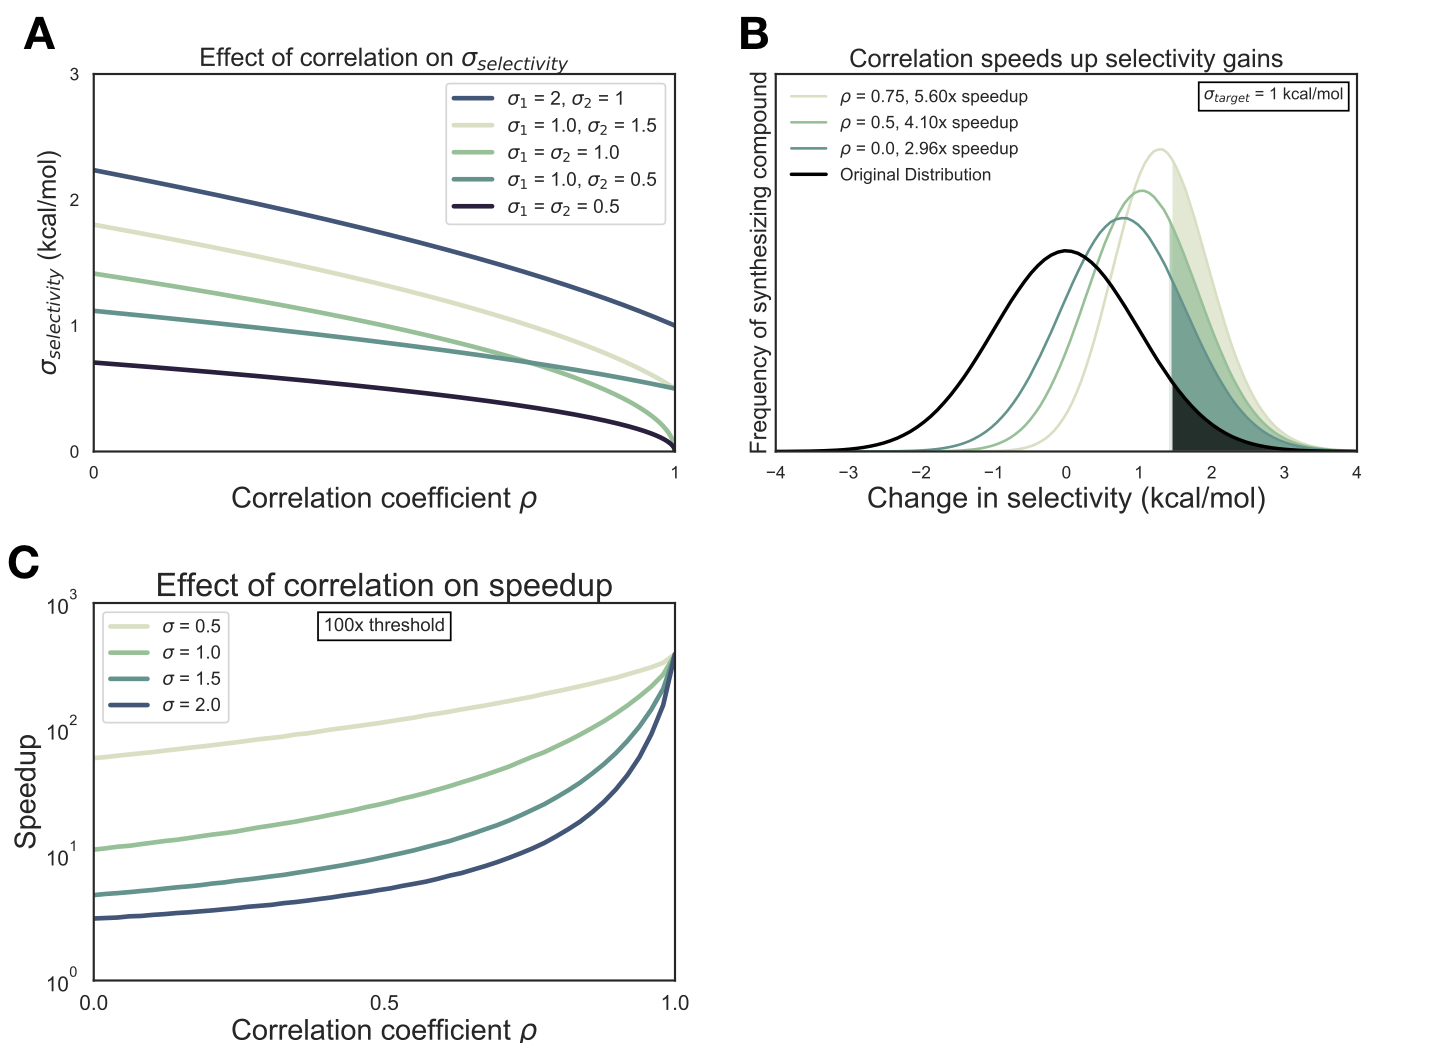
\includegraphics[width=0.9\textwidth]{figures/figure1.png}
  \caption[Free energy calculations speed up selectivity optimization]{{\bf Free energy calculations speed up selectivity optimization} ({\bf A})  The effect of correlation on expected errors for predicting selectivity ($\sigma_{selectivity}$) in kcal/mol. Each curve represents a different combination of target errors ($\sigma_1$ and $\sigma_2$). ({\bf B}) The change in selectivity for molecules proposed by medicinal chemists optimizing a lead candidate can be modeled by a normal distribution centered on 0 with a standard deviation of 1 kcal/mol (black curve). Each green curve corresponds to the distribution of compounds made after screening for a 1 log unit (1.4 kcal/mol) improvement in selectivity with a free energy methodology with a 1 kcal/mol per target error and a particular correlation. The shade region of each curve corresponds to the compounds with a real 1 log unit  improvement in selectivity. The speed up is calculated as the ratio of the percentage of compounds made with a real 1 log unit improvement to the percentage of compounds that would be expected in the original distribution.  ({\bf C}) The speedup (y-axis, log scale) expected for 100x (2 log units, 2.8 kcal/mol) selectivity optimization as a function of correlation coefficient $\rho$. Each curve corresponds to a different $\sigma_{target}$ value.
  }
 \label{fig:figure-1}
\end{figure}
\end{landscape}

\subsection{The CDK2 and CDK9 experimental dataset demonstrates the difficulty in achieving selectivity for closely related kinases}

To begin quantifying the correlation of errors in free energy predictions for selectivity, we set out to gather datasets that met a number of criteria. We looked for datasets that contained binding affinity data for a number of kinase targets and ligands, as well as having crystal structures for each target with the same co-crystallized ligand. For the CDK2/CDK9 datatset~\citep{Shao2013-oe}, ligand 12c was cocrystallized with CDK2/cylin A (Figure~\ref{fig:figure-2}A, left) and CDK9/cyclin T (Figure~\ref{fig:figure-2}B, left), work that was published in a companion paper~\citep{Hole2013-sr}. In both CDK2 and CDK9, ligand 12c forms relatively few hydrogen bond interactions with the kinase. Each kinase forms a set of hydrogen bonds between the ligand scaffold and a hinge residue (C106 in CDK9 and L83 in CDK2) that is conserved across all of the ligands in this series. CDK9, which has slightly lower affinity for ligand 12c (Figure~\ref{fig:figure-2}C, right), forms a lone interaction between the sulfonamide of ligand 12c and residue E107. On the other hand, CDK2 forms interactions between the sulfonamide of ligand 12c and residues K89 and H84. The congeneric series of ligands contains a number of challenging perturbations, particularly at substituent point R3 (Figure~\ref{fig:figure-2}C, left). Ligand 12i also presented a challenging perturbation, moving the 1-(piperazine-1-yl)ethanone from the \emph{meta} to \emph{para} location. 

This congeneric series of ligands also highlights two of the challenges of working from publicly available data. First, the dynamic range of selectivity is incredibly narrow, with a mean $\Delta \Delta G_{selectivity}$ (CDK9 - CDK2) of only -0.65 kcal/mol, and a standard deviation of 0.88 kcal/mol. Additionally, experimental uncertainties are not reported for the experimental measurements. Thus, for this and subsequent sets of ligands, the experimental uncertainty is assumed to be 0.3 kcal/mol based on previous work done to summarize uncertainty in experimental data~\citep{BROWN2009420,Hauser:2018vz}. 
\begin{landscape}
\begin{figure}[p]
\centering
	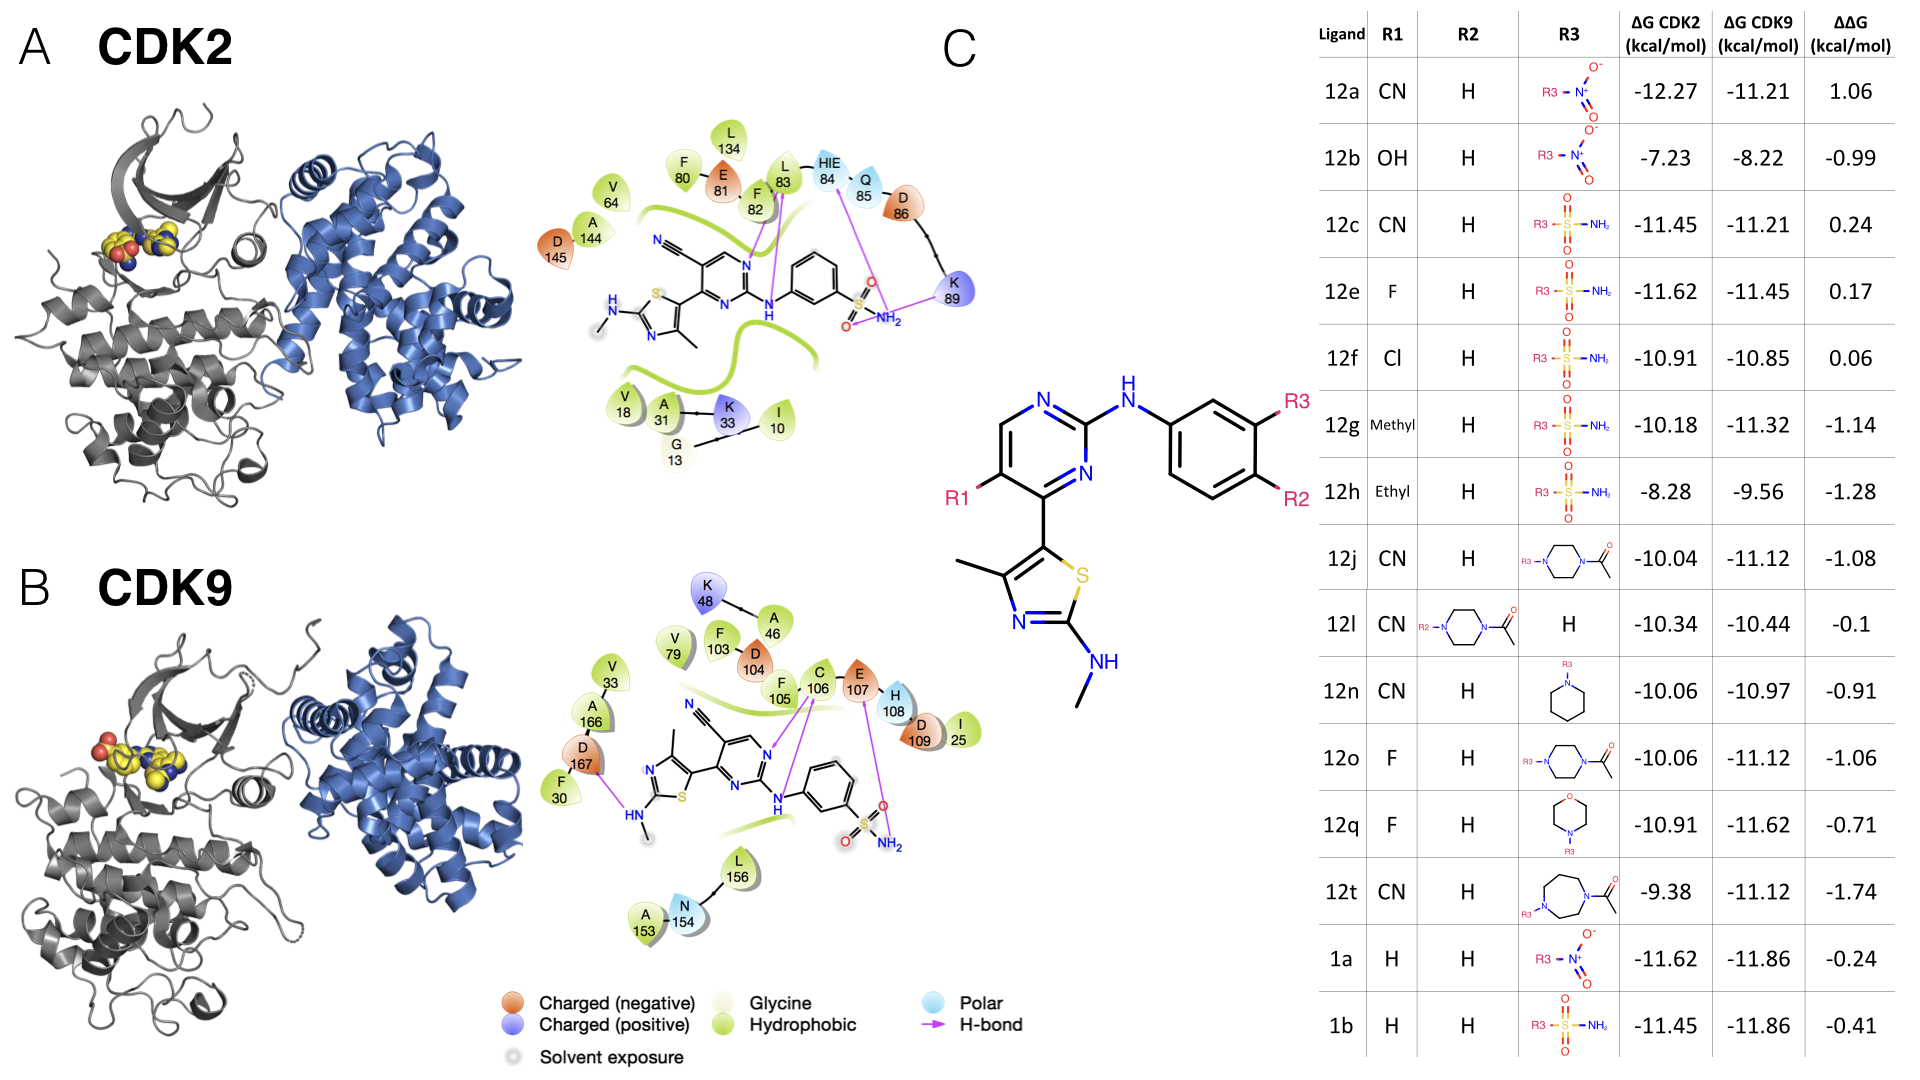
\includegraphics[width=1.0\linewidth]{figures/figure2.png}
	\caption[A CDK2/CDK9 selectivity dataset from Shao et \emph{al}., 2013]{{\bf A CDK2/CDK9 selectivity dataset from Shao \emph{et al.,} 2013}
({\bf A})  \emph{(left)} Crystal Structure (4BCK)\citep{Hole2013-sr} of CDK2 (gray ribbon)  bound to ligand 12c (yellow spheres). Cyclin A is shown in blue ribbon \emph{(right)} 2D ligand interaction map of ligand 12c in the CDK2 binding site. 
({\bf B}) \emph{(left)} Crystal structure of CDK9 (4BCI)\citep{Hole2013-sr} (gray ribbon) bound to ligand 12c (yellow spheres). Cyclin T is shown in blue ribbon. \emph{(right)} 2D ligand interaction map of ligand 12c in the CDK9 binding site.
({\bf C}) \emph{(left)} 2D structure of the common scaffold for all ligands in congeneric ligand series 12 from the publication \emph{(right)} A table summarizing all R group substitutions as well as the published experimental binding affinities and selectivities\citep{Shao2013-oe}. 
	}
	\label{fig:figure-2}
\end{figure}
\end{landscape}

\subsection{The CDK2 and ERK2 dataset achieves higher levels of selectivity for more distantly related kinases}
\todo{I probably need to either remove the reference to how closely related the kinases are, or come up with a way to quantify that - SKA}
The CDK2/ERK2 datatset from Blake \emph{et al.,} 2016 also met the criteria described above. Crystal structures for both CDK2 (Figure~\ref{fig:figure-3}A, top) and ERK2 (Figure~\ref{fig:figure-3}B, top) were available with ligand 22 co-crystallized. Of note, CDK2 was not crystallized with cyclin A, despite cyclin A being include in the affinity assay reported in the paper~\citep{Blake2016-su}. CDK2 adopts a DFG-in conformation with the $\alpha$C helix rotated out, away from the ATP binding site and breaking the conserved salt bridge between K33 and E51 (Supp. Figure~\ref{fig:sup-figure-1}A), indicative of an inactive kinase~\citep{Huse2002-ml,Hari:2013dp}. By comparison, the CDK2 structure from the CDK2/CDK9 dataset adopts a DFG-in conformation with the $\alpha$C helix rotated in, forming the ionic bond between K33 and E51 indicative of an active kinase, due to allosteric activation by cyclin A. While missing cyclins have caused problems for free energy calculations in prior work~\todo{is there a good citation for this?}, it is possible that the fully active conformation contributes equally to binding affinity for all of the ligands in the series, and the high accuracy of the potency predictions (Figure~\ref{fig:figure-4}, top left) is the result of fortutious cancellation of errors. The binding mode for this series is similar between both kinases. There is a set of conserved hydrogens bonds between the scaffold of the ligand and the backbone of one of the hinge residues (L83 for CDK2 and M108 for ERK2). The conserved lysine (K33 for CDK2 and K54 for ERK2), normally involved in the formation of a ionic bond with the $\alpha$C helix, forms a hydrogen bond with the scaffold (Figure~\ref{fig:figure-4}A and~\ref{fig:figure-4}B, bottom) in both CDK2 and ERK2. However, in the ERK2 structure, the hydroxyl engages a crystallographic water as well as N154 in a hydrogen bond network that is not present in the CDK2 structure. 
The congenric ligand series features a single subsituent point, with the R groups exposed to the solvent. This helps explain the extremely narrow distribution of selectivities, with a mean selectivity of -1.74 kcal/mol (ERK2 - CDK2) and standard deviation of 0.56 kcal/mol. This suggests that the selectivity is largely driven by the scaffold and unaffected by the R group substitutions.

\begin{landscape}
\begin{figure}[p]
\centering
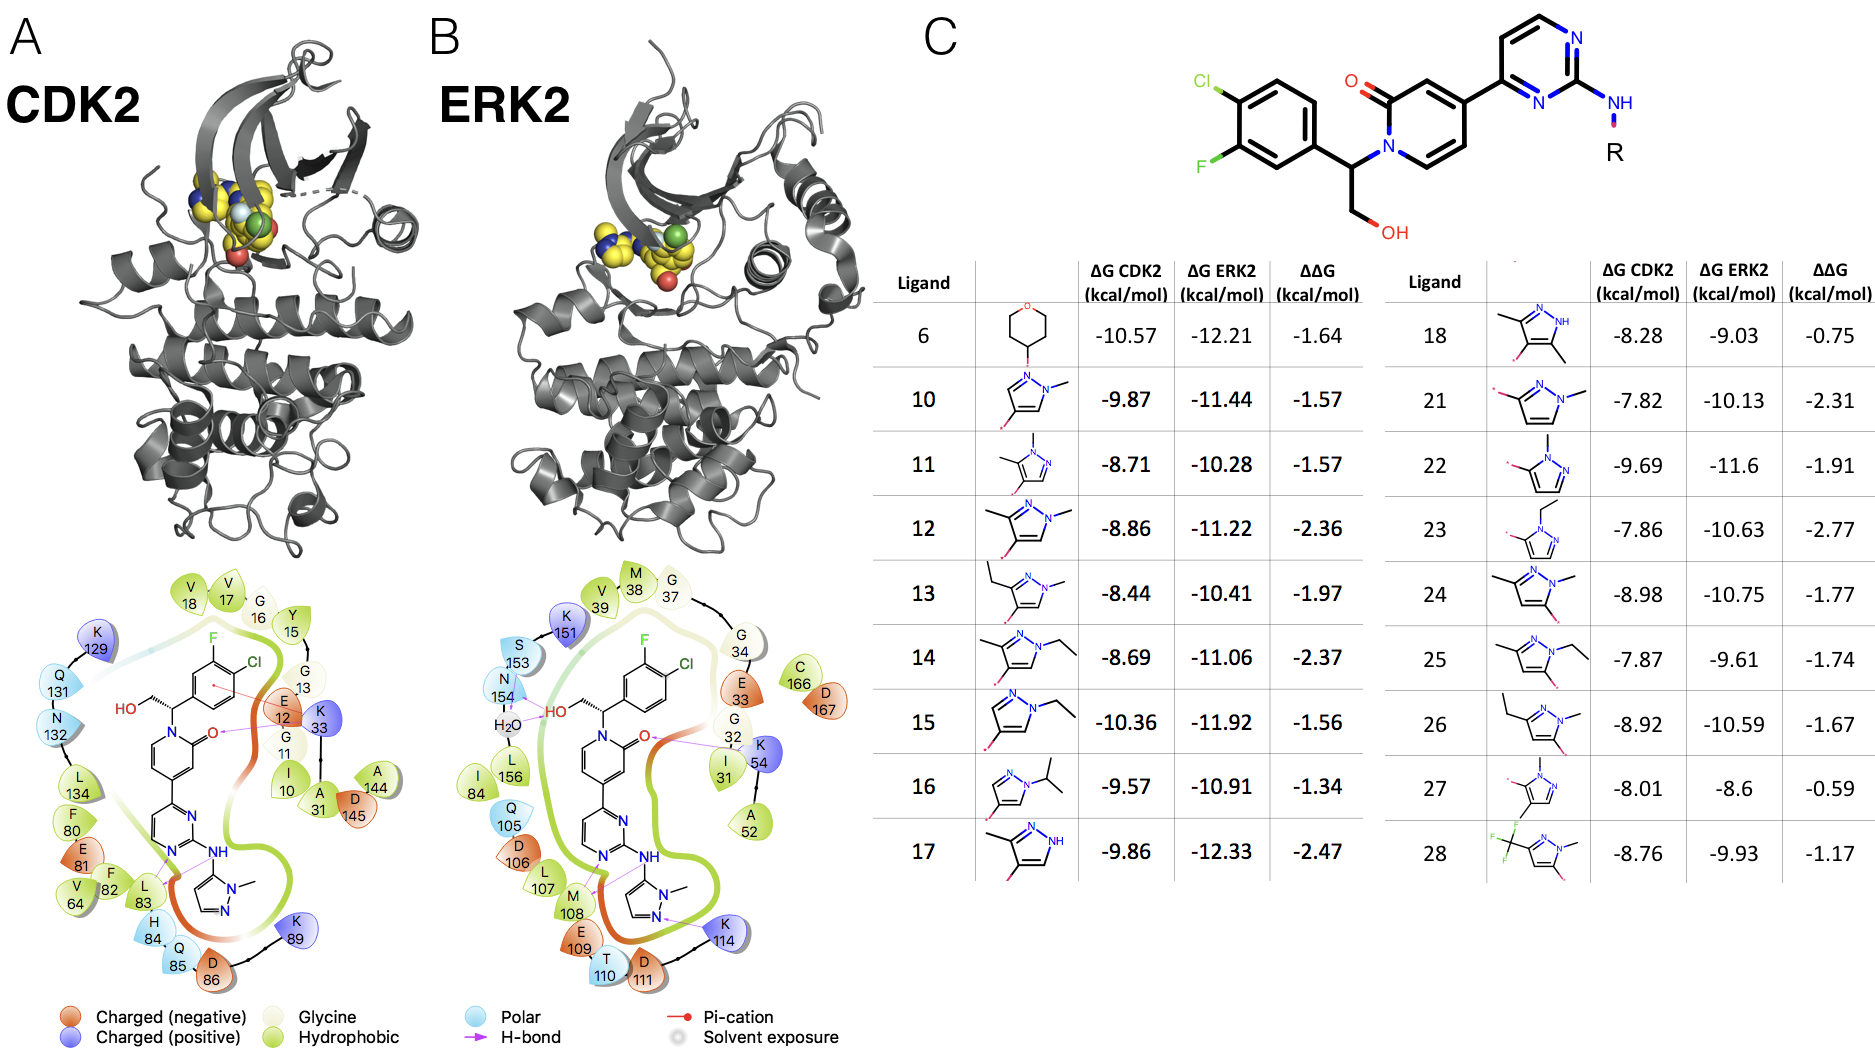
\includegraphics[width=1.0\linewidth]{figures/figure3.png}
\caption[CDK2 and ERK2 selectivity dataset from Blake et \emph{al}., 2016]{
{\bf CDK2 and ERK2 selectivity dataset from Blake et \emph{al}., 2016} \\
({\bf A})  \emph{(top)} Crystal structure of CDK2 (5K4J) shown in gray cartoon and ligand 22 shown in yellow spheres. \emph{(bot)} 2D interaction map of ligand 22 in the binding pocket of CDK2
({\bf B}) \emph{(top)} Crystal structure of ERK2 (5K4I) shown in gray cartoon with ligand 22 shown in yellow spheres. \emph{(bot)} 2D interaction map of ligand 22 in the binding pocket of ERK2.
({\bf C}) \emph{(top)} Common scaffold for all of the ligands in the Blake dataset, with R denoting attachment side for substitutions. \emph{(bot)} Table showing R group substitutions and experimentally measured binding affinities and selectivities. Ligand numbers correspond to those used in publication. 
}
\label{fig:figure-3}
\end{figure}
\end{landscape}

\subsection{FEP+ calculations show accurate potency predictions for ERK2/CDK2 and larger errors for CDK2/CDK9}
The FEP+ predictions of single target potencies ($\Delta G$) showed good accuracy for the CDK2 and ERK2 dataset (Figure~\ref{fig:figure-4}, top), with an RMSE of $0.37^{0.57}_{0.16}$ and $0.53^{0.81}_{0.22}$ kcal/mol, respectively. All of the CDK2 and ERK2 potencies were predicted within 1 log unit of the experimental value. Despite the high accuracy for the single target potency predictions, the selectivity ($\Delta \Delta G_{selectivity}$) predictions show an RMSE of $0.81^{1.26}_{0.37}$ kcal/mol, with all of the predictions falling within 1 log unit of the experimental values (Figure~\ref{fig:figure-4}, top right panel).\todo{this will change if we take of the ff uncertainty error bars}. Despite the high accuracy of the predictions, the narrow dynamic range and high uncertainty from experiment and calculation obscures any signal in the data. 
The CDK2 and CDK9 datasets show higher errors in the potency predictions, with an RMSE of $1.39^{2.05}_{0.58}$ and $1.71^{2.61}_{0.61}$ kcal/mol respectively. There are a number of outliers that fall outside of 1 log unit from the experimental value. While the higher per target errors make predicting potency more difficult, the selectivity predictions show a much lower RMSE of $0.74^{1.25}_{0.31}$ kcal/mol. This suggests that some correlation in the error is leading to fortuitous cancellation of systematic error, leading to more accurate than expected predictions of $\Delta \Delta G_{selectivity}$. 

\begin{landscape}
\begin{figure}
\centering
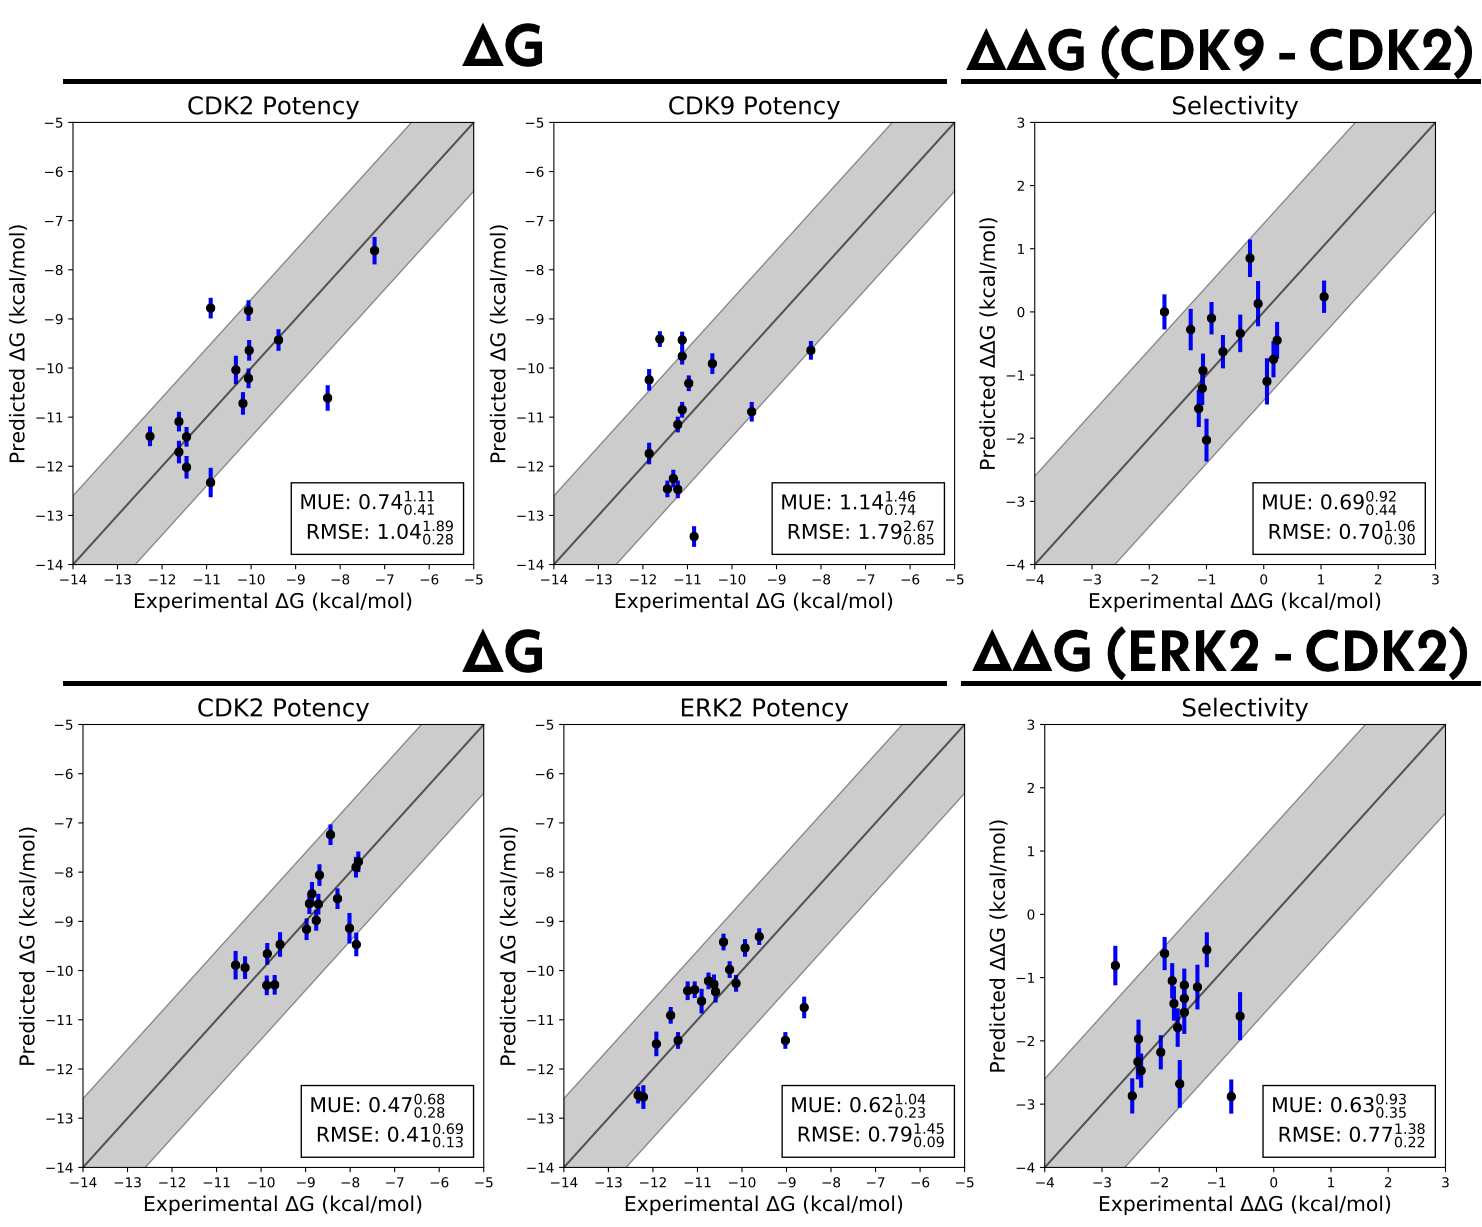
\includegraphics[width=0.6\linewidth]{figures/figure4.png}
\caption[Relative free energy calculations can accurately predict potency, but show larger errors for selectivity predictions.]{
{\bf Relative free energy calculations can accurately predict potency, but show larger errors for selectivity predictions.} \\
Single target potencies and selectivities for CDK2/ERK2 from the Blake datasets (\emph{top}), and CDK2/CDK9 (\emph{bottom}) from the Shao datasets. The experimental values are shown on the X-axis and calculated values on the Y-axis. Each data point corresponds to a ligand for a given target. All values are shown in units of kcal/mol. The horizontal error bars show the assumed experimental uncertainty of 0.3 kcal/mol\citep{BROWN2009420}. To better highlight outliers that are unlikely due simply to forcefield errors, we presume the forcefield error ($\sigma_\mathrm{FF} \approx$ 0.9 kcal mol$^{-1}$~\cite{Harder:J.Chem.TheoryComput.:2016}) also behaves as a random error. We show the total estimated statistical and forcefield error ($\sqrt{\sigma_\mathrm{FF}^2 + \sigma_\mathrm{calc}^2}$) as vertical blue error bars. The black vertical error bars correspond to the statistical error ($\sigma_{calc}$). The black line indicates agreement between calculation and experiment, while the gray shaded region represent 1.36 kcal/mol (or 1 log unit) error. The MUE and RMSE are shown on each plot with bootstrapped 95$\%$ confidence intervals.
}
\label{fig:figure-4}
\end{figure}
\end{landscape}

\subsection{Free energy calculation errors are correlated, accelerating selectivity optimization}
To quantify the correlation coefficient ($
\rho$) of the errors in our calculations, we built a Bayesian graphical model, as described in the methods section. Briefly, we modeled the absolute free energy ($G$) of each ligand in each phase (complex and solvent) as in equation~\ref{eq4}. The model was chained to the FEP+ calculations by providing the $\Delta G^{calc}_{phase,ij,target}$ as observed data, as in equation~\ref{eq6}. As in equation, the experimental data was modeled as a normal distribution centered around the true free energy of binding ($\Delta G^{true}_{i,target}$) corrupted by experimental error, which is assumed to be 0.3 kcal/mol from previous work done to quantify the uncertainty in publicly available data~\citep{BROWN2009420}. The reported IC50 values from each dataset were treated as data observations (Equation~\ref{eq12}) and the $\Delta G^{true}_{i,target}$ was assigned a weak normal prior (Equation~\ref{eq13}). The correlation coefficient was calculated for each sample according to equation~\ref{eq9}. 
The correlation coefficient $\rho$ for the CDK2/ERK2 calculations was quantified to be $0.5^{0.33}_{-0.23}$, indicating that the errors are largely uncorrelated between ERK2 and CDK2 (Figure~\ref{fig:figure-5}A, right). The joint marginal distribution of the error ($\epsilon$) for each target is symmetric, which is expected for cases in which $\rho$ is 0 (Supp. Figure~\ref{fig:sup-figure-2}). Despite the weak correlation in errors, the high per target accuracy of these calculations should have a 2-3x speed up for 1 log unit selectivity optimization, and a 20-30x speed up for 2 log unit selectivity optimization (Figure~\ref{fig:figure-5}A, right). 
The CDK2/CDK9 calculations show strong evidence of correlation, with a correlation coefficient of $0.70^{0.82}_{0.57}$ (Figure~\ref{fig:figure-5}B, right). The joint marginal distribution of errors is strongly diagonal, which is expected based on the value for $\rho$ (Figure~\ref{fig:figure-5}B, left). The high correlation in errors leads to a speed up of 4-5 for 1 log unit selectivity optimization and 30-40x for 2 log unit selectivity optimization (Figure~\ref{fig:figure-5}B, right), despite the much higher per target errors.
Quantifying $\rho$ for these calculations enables estimation of $\sigma_{selectivity}$, which is useful for estimating expected error for prospective studies, where the experimental values for $\Delta \Delta G_{selectivity}$ are not yet known. Based on the distribution quantified for $\rho$, the expected $\sigma_{selectivity}$ for the CDK2/CDK9 calculations is between 0.76 and 1.16 kcal/mol (Supp. Figure~\ref{fig:sup-figure-3}), which is in good agreement with the bootstrapped RMSE (Figure~\ref{fig:figure-4}, bottom). For the CDK2/ERK2 calculations, $\sigma_{selectivity}$ is expected to fall between 0.82 kcal/mol and 1.10 kcal/mol (Supp. Figure~\ref{fig:sup-figure-3}), which is also in good agreement with the bootstrapped RMSE (Figure~\ref{fig:figure-4}, top). 

\begin{landscape}
\begin{figure}
\centering
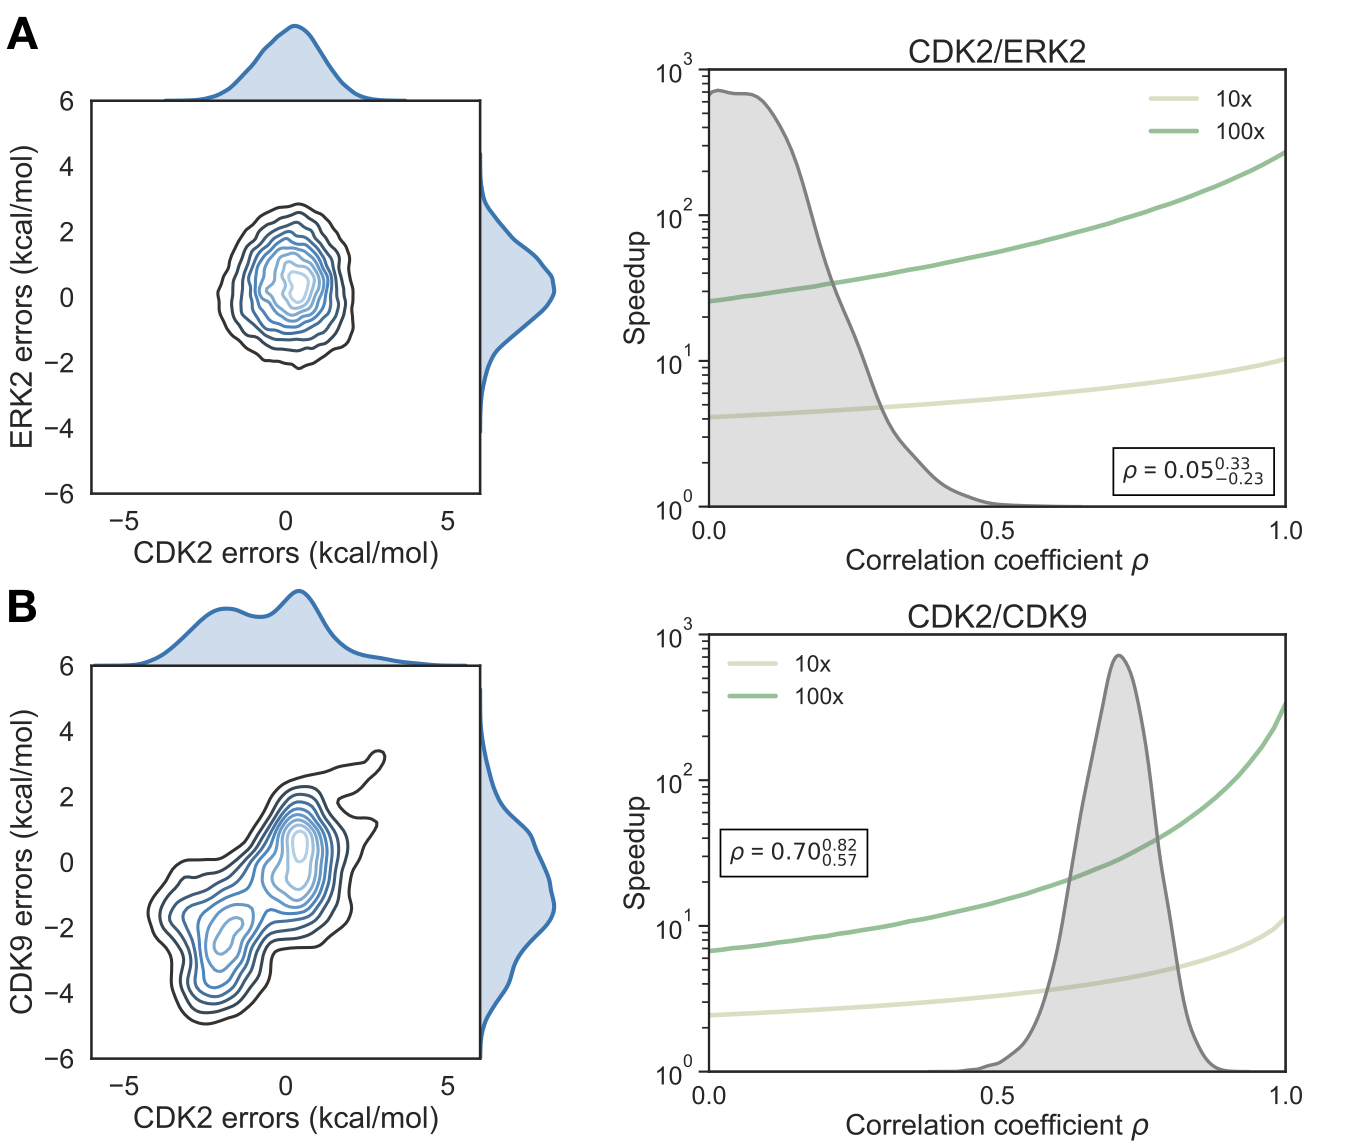
\includegraphics[width=0.7\linewidth]{figures/figure5.png}
\caption[Correlation in selectivity prediction errors can be used to accelerate selectivity optimization]{
{\bf Correlation in selectivity prediction errors can be used to accelerate selectivity optimization} \\
({\bf A}) (\emph{left}) The joint posterior distribution of the prediction errors for CDK2 (X-axis) and ERK2 (Y-axis) from the Bayesian graphical model. (\emph{right}) Speedup in selectivity optimization (Y-axis) as a function of correlation coefficient (X-axis). The posterior marginal distribution of the correlation coefficient ($\rho$) is shown in gray, while the expected speed up is shown for 100x (green curve) and 10x (yellow curve) selectivity optimization. The inserted box shows the mean and 95\% confidence interval for the correlation coefficient. 
({\bf B}) (\emph{left}) The same as above, with CDK2 (X-axis) and CDK9 (Y-axis). (\emph{right}) As above, for the CDK2/CDK9 calculations.
}
\label{fig:figure-5}
\end{figure}
\end{landscape}

\section{Discussion and Conclusions}
We have demonstrated, using a simple numerical model, the impact that free energy calculations with even weakly correlated errors can have on speeding up the optimization of selectivity in small molecule kinase inhibitors. While the expected speed up is dependent on the per target error of the method ($\sigma_{target}$), the speedup is also highly dependent on the correlation of errors made for both targets. Unsurprisingly, free energy methods have greater impact as the threshold for selectivity optimization goes from 10x to 100x. While 100x selectivity optimization is difficult to achieve, the expected benefit from free energy calculations is also quite high, with 1 and 2 order of magnitude speedups possible. 
To quantify the correlation of errors in two example systems, we gathered experimental data for two congeneric ligand series with experimental data for CDK2 and ERK2, as well as CDK2 and CDK9. These datasets, which had crystal structures for both targets with the same ligand co-crystallized, are exemplify the difficulty in predicting selectivity. The dynamic range of selectivity for both systems is incredibly narrow, with most of the perturbations not having a major impact on the overall selectivity achieved. Furhter, the data was reported with unrelaible experimental uncertainties, which makes quantifying the errors made by the free energy calculations difficult. This issue is common when considering selectivity, as many kinase-oriented high throughput screens are carried out at a single concentration and not highly quantitative. Work is being done to increase the availability of publicly available, high quality biophysical data for selectivity measurements, which will benefit future work on predicting selectivity using physical models and machine learning techniques. 
\todo[inline]{insert a discussion of outliers in the FEP+ calculations here?}
\todo[inline]{discuss quantification of rho (is there a way to know a priori what rho might be?)}
\todo[inline]{discussion of the expected speedup and sigma based on the quantification of rho}
\todo[inline]{extensions include: separating statistical error (unless this gets added into the results section}
\todo[inline]{Do we want to mention protein mutation FEP+ to enable cycle closure analysis for certain highly related targets?}

\begin{landscape}
\begin{figure}[p]
\centering
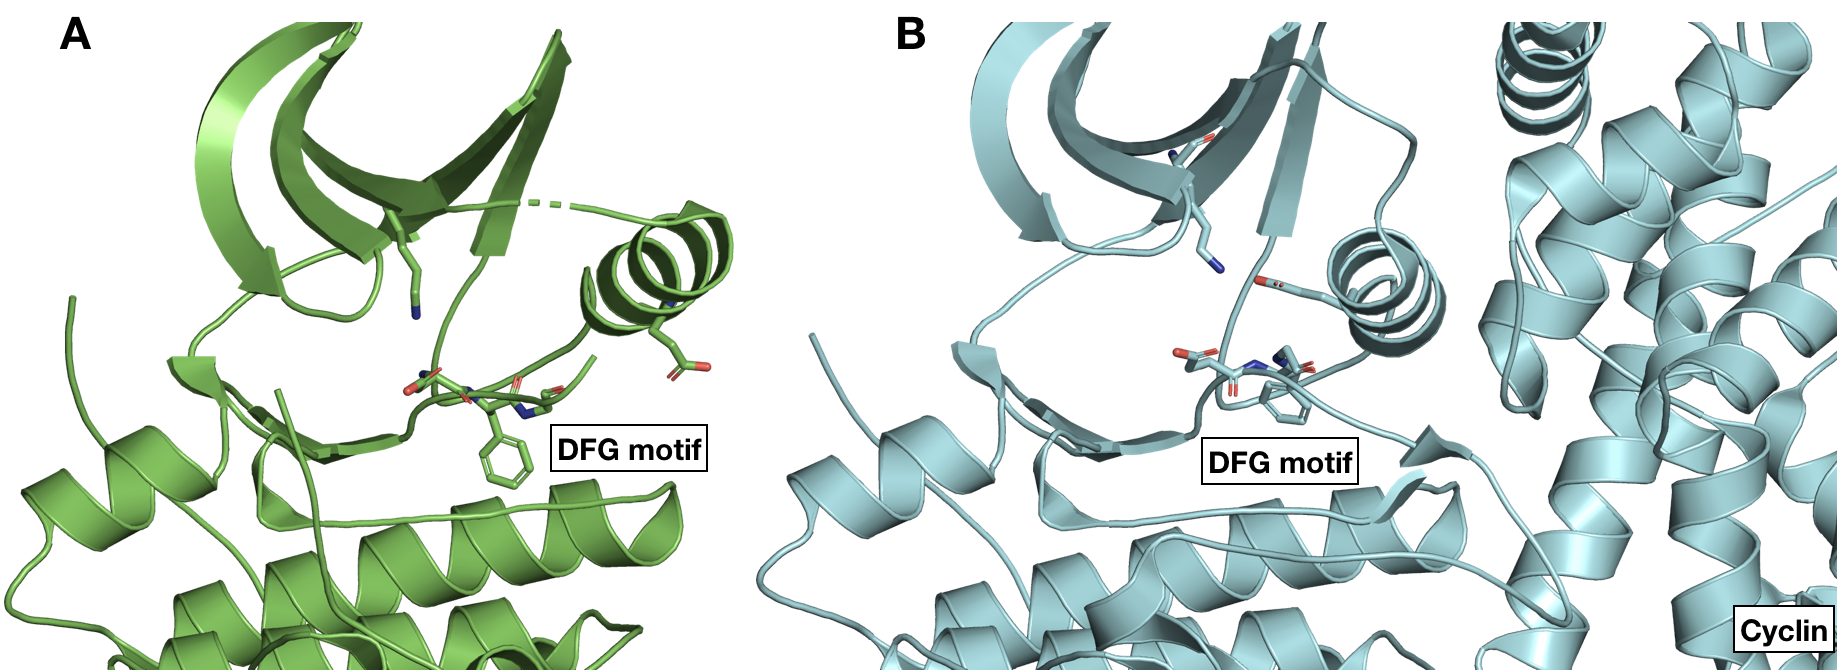
\includegraphics[width=1.0\linewidth]{figures/supp_figure1.png}
\caption[CDK2 adopts an inactive conformation in the crystal structure used for the CDK2/ERK2 calculations]{
{\bf CDK2 adopts an inactive conformation in the crystal structure used for the CDK2/ERK2 calculations} 
({\bf A}) CDK2 (5K4J) adopts an inactive conformation in the absence of its cyclin. The DFG motif is in a DFG-in conformation, with the $\alpha$C helix rotated outwards, breaking the salt bridge between K33 and E51 (Uniprot numbering) that is typically a marker of an active conformation. Notably, the Phe in the DFG motif does not completely form the hydrophobic spine due to the rotation of the $\alpha$C helix~\citep{Hu:2015kh}
({\bf B}) The CDK2 structure used for the CDK2/CDK9 calculations (4BCK) contains cyclin A and adopts a DFG-in/$\alpha$C helix-in conformation that forms the salt bridge between K33 and E51. This is typically indicative of a fully active kinase~\citep{Huse2002-ml,Hari:2013dp}. 
}
\label{fig:sup-figure-1}
\end{figure}
\end{landscape}

\begin{landscape}
\begin{figure}[p]
\centering
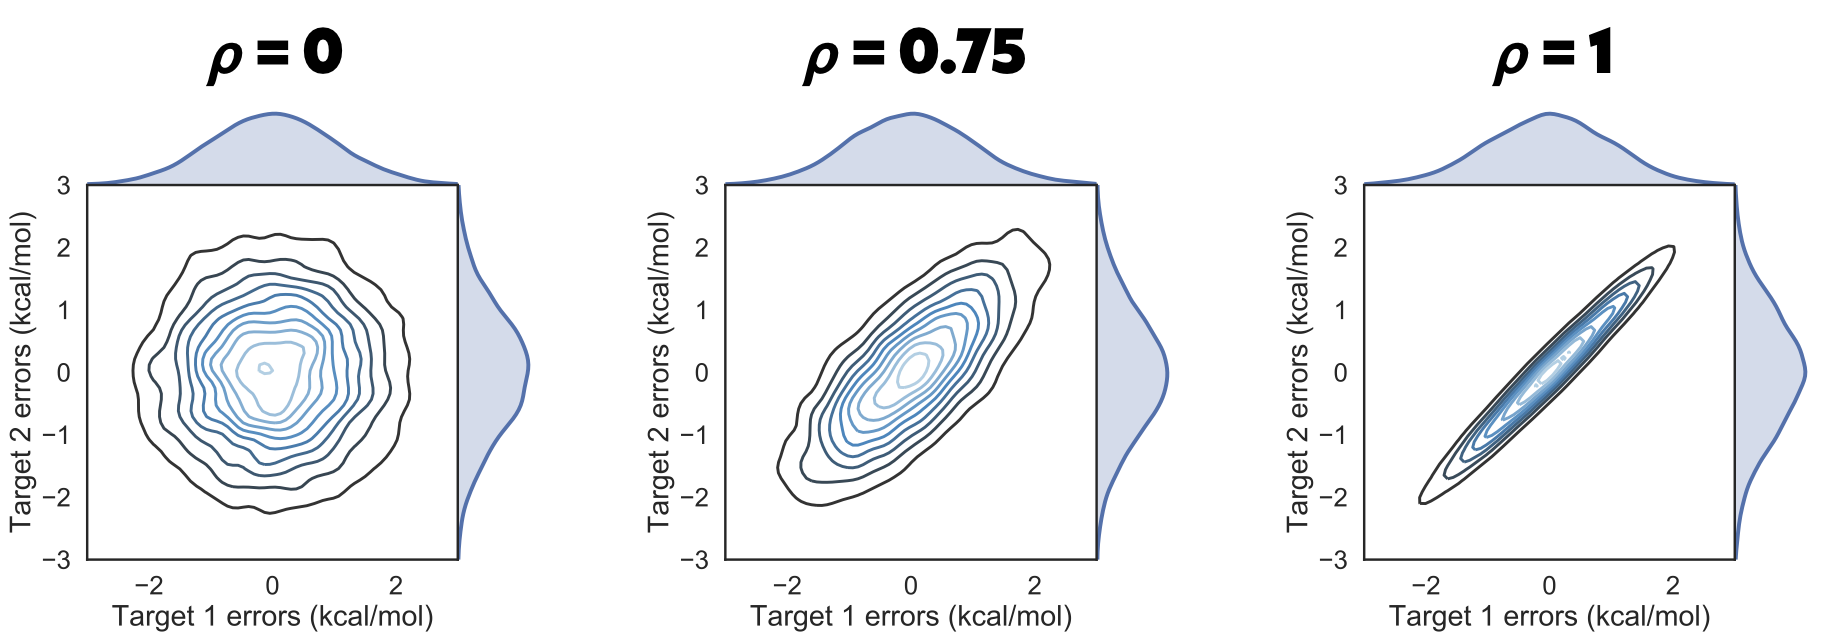
\includegraphics[width=1.0\linewidth]{figures/supp_2.png}
\caption[ Correlation coefficient $\rho$ controls the shape of the joint marginal distribution of errors]{
{\bf Correlation coefficient $\rho$ controls the shape of the joint marginal distribution of errors} 
As $\rho$ increases, the joint marginal distribution of errors become more diagonal. Each panel shows 10000 samples drawn from a multivariate normal distribution centered around 0 kcal/mol, where the per target error was set to 1 kcal/mol and $\rho$ to the value indicated in bold over the plot. 
}
\label{fig:sup-figure-2}
\end{figure}
\end{landscape}

\begin{landscape}
\begin{figure}[p]
\centering
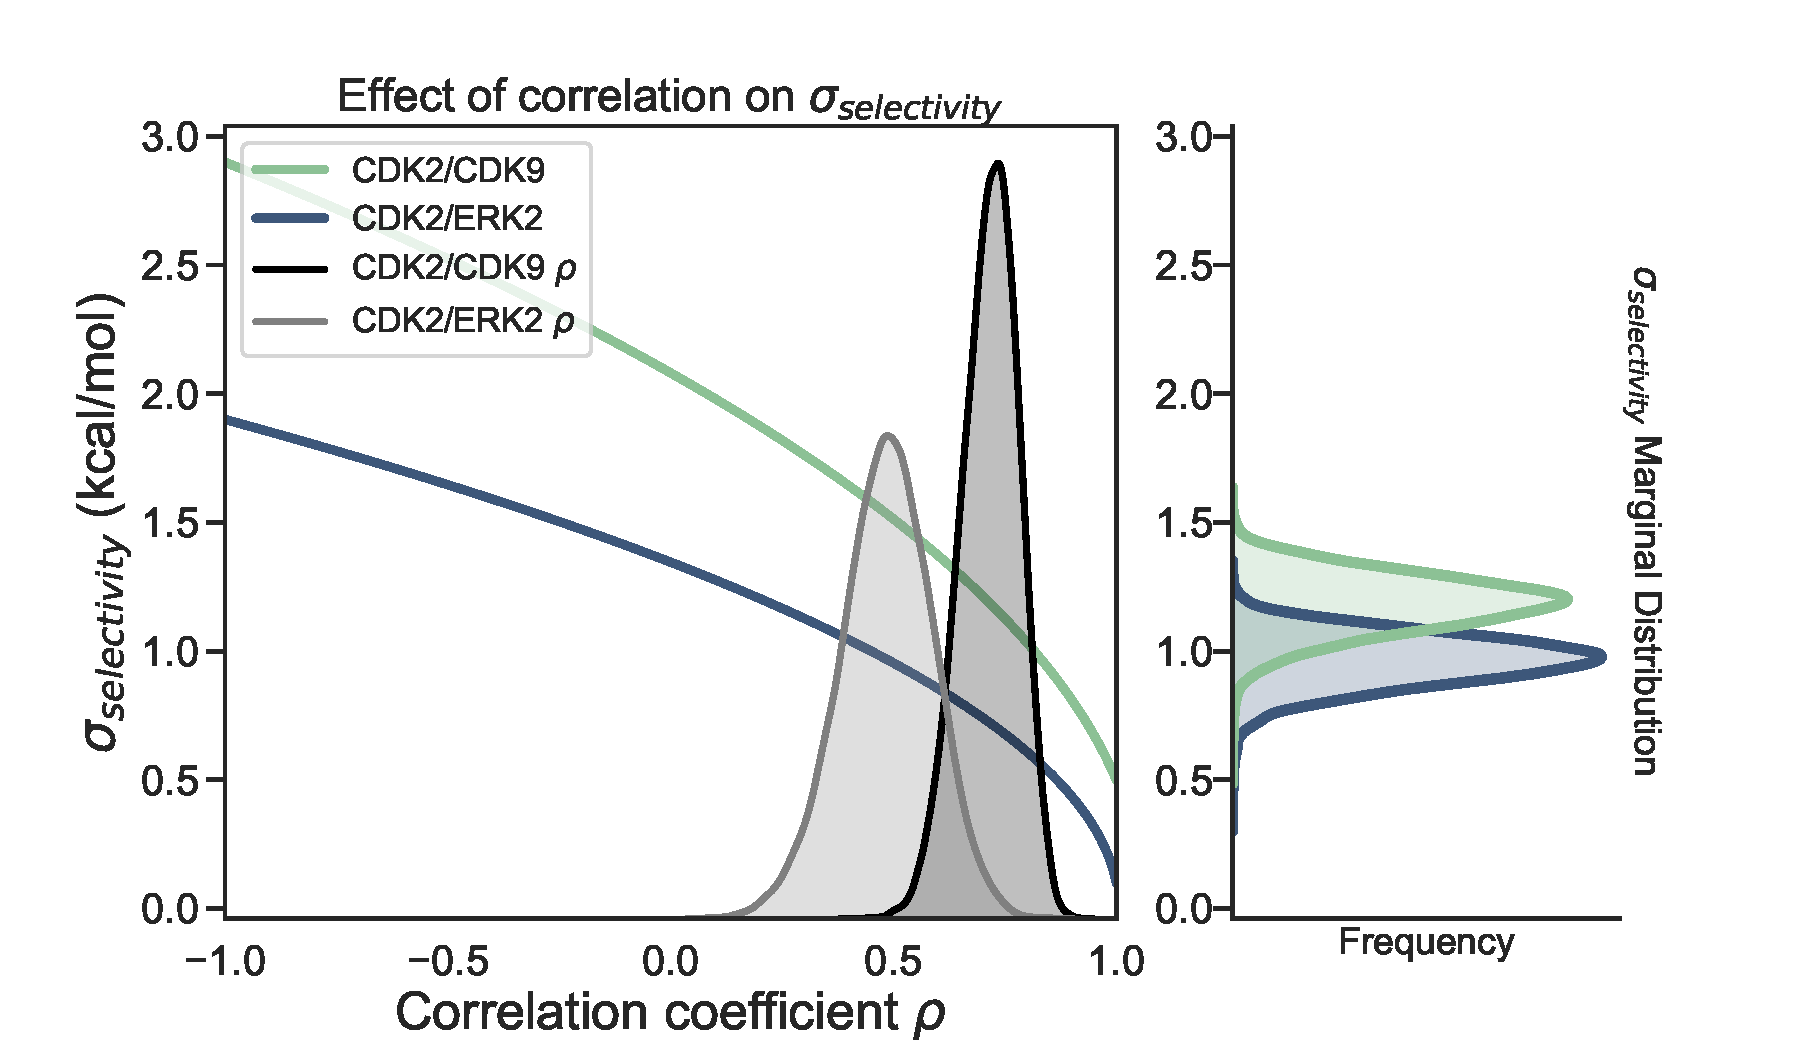
\includegraphics[width=0.8\linewidth]{figures/supp_figure3.pdf}
\caption[Correlation reduces the expected error for selectivity predictions]{
{\bf Correlation reduces the expected error for selectivity predictions}
As corelation coefficient $\rho$ increases, $\sigma_{selectivity}$ decreases. The intersection between CDK2/CDK9 $\sigma_{selectivity}$ (green curve) and $\rho$ (black distribution) indicates the range of expected $\sigma_{selectivity}$ values. The intersection for CDK2/ERK $\sigma_{selectivity}$ (blue curve) and $\rho$ (gray distribution) suggests the expected $\sigma_{selectivity}$ range for that set of calculations. 
}
\label{fig:sup-figure-3}
\end{figure}
\end{landscape}

\chapter{Understanding the functional impact of mTOR clinical kinase mutations using physical modeling}

\section{Introduction}
\subsection{mTOR forms the catalytic core of protein complexes that control a number of cellular processes}
mTOR (mammalian target of rapamycin) is a serine-threonine kinase that controls a number of cellular processes~\citep{Laplante:2012fm,Saxton:2017cv} by integrating signaling from the MAPK and PI3K pathways~\citep{Mendoza2011-bj}. mTOR forms the catalytic core of heteromeric protein complexes, mTORC1 and mTORC2, that differ in the regulatory proteins that decorate the kinase. mTORC1 is defined by RAPTOR~\citep{Kim:2002vh,Hara:2002tn} and PRAS40~\citep{Yang:2017gu}, while mTORC2 is characterized by RICTOR~\citep{Sarbassov:2004kv}. Each complex contains a number of shared regulatory proteins, such as mLST8~\cite{BarPeled:2012gq} and DEPTOR~\citep{Peterson:2009fc}. mTOR itself is an atypical kinase, and includes a number of insertions that deviate from the canonical kinase fold. The C-terminal fragment crystal structure (Figure~\ref{fig:mtor-figure1})shows that the kinase domain is hugged by a FAT domain~\citep{Yang:2013gaa}, forming a C-shaped clamp around the kinase domain. The FAT domain forms a number of regulatory salt bridges that have been implicated in controlling the activity of the kinase~\cite{Yang:2013gaa}. The FK506-rapamycin-binding (FRB) domain hangs over the opening cleft to the active site~\cite{Yang:2013gaa} (Figure~\ref{fig:mtor-figure1}). The FRB domain is exposed in mTORC1, while is it thought to be occluded and inaccesible to FKBP12 in mTORC2~\citep{Gaubitz:2015gr}. Complex activity is hypothesized to be regulated via restricted access to the active site by architectural elements as well as rapalog-mediated recruitment of FKBP to the FRB domain~\citep{Aylett:2016gs}. 

\begin{landscape}
	\begin{figure}[p]
		\centering
		\includegraphics[width=0.8\linewidth]{figures/mtor-fig1.pdf}
		\caption[mTOR is an atypical kinase with a number of regulatory domains]{
			{\bf mTOR is an atypical kinase with a number of regulatory domains}
			mTOR (PDBID: 4JSV) is shown as a cartoon diagram. The kinase domain (white) has a number of structural features highlighted, such as the activation loop (teal) as well as a network of regulatory $\alpha$ helices (red) in the active site. The FAT domain (black) clamps around the kinase domain and forms a number of salt bridge and hydrophobic contains with the kinase domain. The FRB domain (gold) hangs over the active site clef and is the site of rapalog binding and rapalog-mediate FBKBP recruitment. \bf{This figure reprinted with permission of James Hsieh}
		}
		\label{fig:mtor-figure1}
	\end{figure}
\end{landscape}

mTORC1 controls a number of biological processes by integrating multiple upstream signals (Figure~\ref{fig:mtor-figure2}). Tuberous sclerosis complex 1/2 (TCS1/2) integrates growth factor signaling from the PI3K/AKT pathway~\citep{Inoki:2002jv,Manning:2002tp} and DNA damage from AMPK~\citep{Jones:2005kg}. TSC1/2 acts as GTPase activating protein (GAP) for RHEB~\citep{Inoki:2003je}, which binds to and activates mTORC1 at the lysosomal surface. mTORC1 localization is controlled by the second major signal it integrates: amino acid availability. Upon stimulation by amino acids, the Ragulator~\citep{BarPeled:2012fr} recruits inactive mTORC1 from the cytosol to the lysosomal surface~\citep{Kim:2008kb,Sancak:2010bu,Efeyan:2012de}, enabling interaction with RHEB. Once active, mTORC1 controls cell growth and protein synthesis by phosphorylating and activating S6K at T389 and inactivating 4EBP1 via a phosphorylation at S65~\citep{Hay:2004ir,Laplante:2012fm}. mTORC1 also activates SREBP1/2, which regulates lipid biosynthesis~\citep{Lamming:2013dza}. mTORC1 activation inhibits autophagy through via ULK1. Recent work suggests that mTORC1 can also control the biophysical properties of the cytoplasm by regulating crowding~\citep{Delarue:2018ca}, impacting the rate of diffusion and expanding the already diverse array of essential processes that mTOR controls. 

\subsection{mTOR is the targeted by inhibitors with two distinct mechanisms of action}
Due to the central role mTOR plays in a wide array of biological processes, it has emerged as the target of extensive drug discovery programs. There are two distinct classes of inhibitors developed to target mTOR: ATP-competitive inhibitors and allosteric inhibitors~\citep{Ballou:2008ec,Lamming:2013kg}. Temsirolimus~\citep{Hudes:2007kp} and Evirolimus~\citep{Motzer:2008cn} are FDA-approved inhibitors~\citep{fda-approved-kinase-inhibitors} that are thought to inhibit mTOR through recruiting FKBP family members, such as FKBP12, to the FRB domain~\citep{Hausch:2013iu}. Evidence suggests FKBP12 recruitment may inhibit mTORC1 activity by inducing a conformational change that prevents S6K binding~\citep{Yip:2010bm}. Further incubation leads to destabilization and disassembly of the protein complex, which is consistent with the time-dependent nature of rapalog inhibition of mTORC1 mediated 4EBP1 phosphorylation~\citep{Yip:2010bm}. The rapalogs are potent inhibitors of mTORC1, while mTORC2 requires chronic rapalog treatment and is highly dependent on FKBP expression levels~\citep{Schreiber:2015fi}. A cryo-EM structure of TORC2 suggests that the FRB domain is inaccessible in TORC2, explaining the relative insensitivity of mTORC2 to rapalog inhibition~\citep{Gaubitz:2015gr}. Rapalogs have also been shown to only partially inhibit mTORC1, often failing to reduce 4EBP phosphorylation levels~\citep{Saxton:2017cv}, despite efficacy at preventing S6K phosphorylation. 
There are an array of ATP-competitive inhibitors developed to target mTOR and other members of the PI3K family of kinases, such as MLN0128~\citep{Slotkin:2015je,Hassan:2014kl}, INK-228 (TAK-128)~\citep{GarciaGarcia:2012jc}, AZD8055~\citep{Chresta:2010ir}, PKI-587~\citep{Mallon:2011gn}, and BEZ-235~\citep{Mukherjee:2012ki}. ATP-competitive inhibitors exhibit a wide range of selectivity, with many inhibiting mTORC1, mTORC2, and multiple isoforms of PI3K. ATP competitive inhibitors target the catalytic activity of mTOR and more fully inhibit mTORC1 and mTORC2 phosphorylation of downstream targets~\citep{Saxton:2017cv}. While many of these inhibitors have struggled clinically due to modest clinical benefits and high toxicity leading to low tolerability~\citep{Pongas:2016jm}, there is considerable excitement about developing mTOR inhibitors to treat a number of diseases. ATP-competitive inhibitor BEZ-235 has shown promising results in preclinical models of lapatinib-resistant PI3K hyperactivated breast cancer~\citep{Eichhorn:2008ff}.  Dual targeted catalytic inhibitors that target both PI3K and mTOR have shown success by abrogating reactivation of Akt, which is caused by the alleviation of negative feedback due to long term treatment with mTOR inhibitors~\citep{RodrikOutmezguine:2011fb}. For example, a dual-inhibitor of mTORC and PI3K$\alpha$, PI-103, showed promising activity against glioma xenografts~\citep{Fan:2006kw}. 

mTOR inhibitors show the most promise in treating diseases with mTOR pathway alterations pathway~\citep{Wagle:2014ej}. Despite initial success, resistance mutations in the FRB or kinase domain have been observed~\citep{Wagle:2014be}. Work has also been done to combine the two mechanisms of action in Rapalink-1, which tethers rapamycin and MLN0128~\citep{RodrikOutmezguine:2016km} with a flexible linker and overcome such acquired resistance. Rapalink also shows improvements over ATP-competitive inhibitors or rapalogs outside of the context of resistance.  In glioblastoma models, ATP-competitive inhibitor MLN0128 and allosteric inhibitor rapamycin showed poor \emph{in vivo} efficacy. In contrast, RapaLink-1, by overcoming poor residence time and potency, was able to durably inhibit mTORC1 and cross the blood-brain barrier~\citep{Fan:2017fk}. 

\begin{landscape}
	\begin{figure}[p]
		\centering
		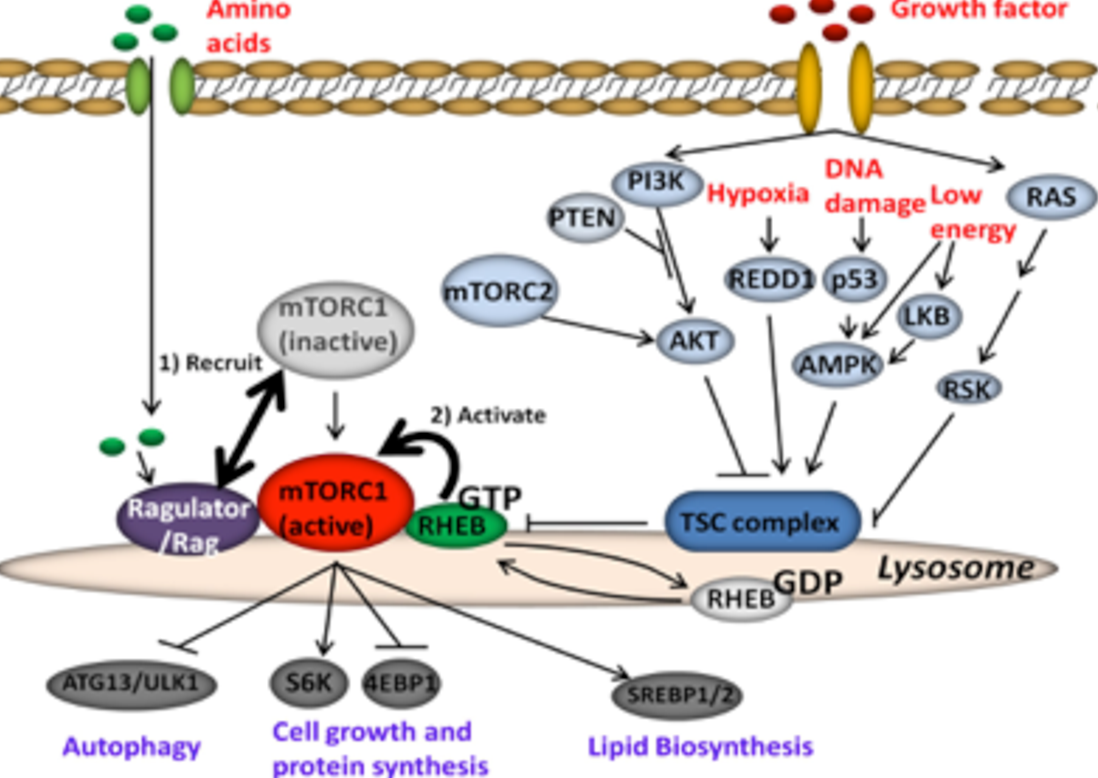
\includegraphics[width=0.8\linewidth]{figures/mtor-fig2.pdf}
		\caption[mTORC1 integrates signaling from a number of inputs]{
			{\bf mTORC1 integrates signaling from a number of inputs}
			The signaling pathway of mTOR involves integrating signaling from the growth factors, amino acids, hypoxia, and DNA damage. Integrating such signals controls the localization and activity of mTORC1, which controls autophagy, cell growth, and macromolecule synthesis through phosphorylation of downstream targets. \bf{This figure courtesy of James Hsieh} 
		}
		\label{fig:mtor-figure2}
	\end{figure}
\end{landscape}

\subsection{mTOR signaling is dysregulated in cancer by hyperactivating missense mutations}
mTOR pathway alterations have been observed in a wide array of cancer types~\citep{Guertin:2007dw} and extensively characterized. Less well studied are missense mutations in mTOR itself. An exceptional responder in a phase 1 clinical trial of pazopanib and everolimus with metastatic urothelial carcinoma lead to the identification of two missense mutations in mTOR~\citep{Wagle:2014ej}, E2014K and E2419K. Subsequent work identified 33 MTOR mutations gathered from publicaly available tumor sequencing data, and found that a number of them activated the mTOR pathway and conferred sensitivity to mTOR inhibitors when engineered into various cancer cell lines \emph{in vitro}~\citep{Grabiner:2014be}. While these missense mutations are pulled from an array of different cancer types, mTOR missense mutations have been observed in about 15\% of clear cell renal cell carcinoma~\citep{CancerGenomeAtlasResearchNetwork:2013ib}. Characterization of these mutations revealed that not only do many of these mutations hyperactivate mTOR (Figure ~\ref{fig:mtor-figure3}), but they can be grouped into complementation groups by determining which double mutations cause hyperactivation at levels higher than the constituent single mutants alone~\citep{Xu:2016fw}. This suggests that these mutations can activate mTOR through different, seemingly complementary mechanisms. 

\begin{landscape}
	\begin{figure}[p]
		\centering
		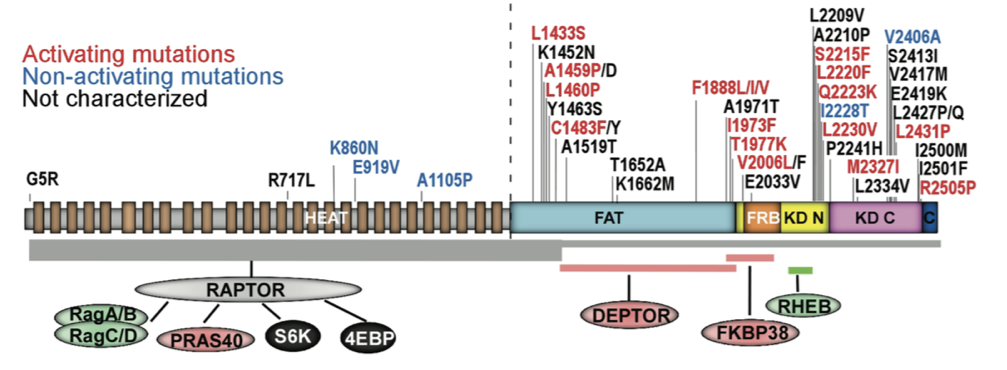
\includegraphics[width=1.0\linewidth]{figures/mtor-fig3.png}
		\caption[Hyperactivating mTOR missense mutations have been observed in cancer]{
			{\bf Hyperactivating mTOR missense mutations have been observed in cancer}
			Diagram shows the domain structure of mTOR, its regulatory interaction partners (negative regulators in pink, positive regu- lators in green, and a dual-role regulator in gray), and the substrates of mTORC1 complex. The positions within mTOR that are involved in the interaction with the regulatory partners are highlighted below the domain structure. The thickness of the horizontal bar of RAPTOR-mTOR interaction indicates the relative binding affinity. mTOR missense mutations derived from ccRCC are mapped and color coded
			to summarize their respective effects on mTORC1 signaling (activating mutations in red). KD N, kinase domain N lobe; KD C, kinase domain C lobe. \bf{This figure reprinted with permission of James Hsieh and the Journal of Clinical investigation~\citep{Xu:2016fw}.}
		}
		\label{fig:mtor-figure3}
	\end{figure}
\end{landscape}

\subsection{Using physical modeling to understand the functional impact of mTOR mutations}
To begin to understand the impact of these missense mutations at an atomistic level, we performed massively parallel molecular dynamics~\citep{Salsbury:2010ij} using the computing resource Folding@Home~\citep{Shirts:2000du}. Molecular Dynamics simulations have been used previously to understand the mechanism of oncogenic and resistance mutations on the structure and activation of EGFR~\citep{Shan:2012bs,Sutto:2013gy}. They have also been applied to understanding missense mutations in p53~\citep{Demir:2011bc}, CLIC2~\citep{Witham:2011co}, opsin~\citep{Tsukamoto:2013gr}, and a host of oncogenes and tumor suppressors\citep{Stehr:2011ga}. Using the previously solved crystal structure~\citep{Yang:2013gaa}, we built models for 45 single, and 190 double mutations, far more than could be crystallized individually~\citep{Xu:2016fw}. We analyzed the simulations for changes in contact formation, as well as changes in order parameters for activation mined from other kinase studies and previous work on mTOR biochemistry. We also piloted alchemical free energy calculations~\citep{Chodera:Curr.Opin.Struct.Biol.:2011} on a number clinically observed mutants, to compute physical testable properties such as change in affinity for ATP-competitive inhibitors and ATP itself. In doing so, we identify promising candidates for resistance mutations to an ATP competitive inhibitor, and lay the ground work for future studies on the application of these methods to studying the functional impact of mutations on inhibitor binding. Taken together, this work forms the beginning of a comprehensive analysis of the impact of these mutations on structure and small molecule binding, which has implications for the treatment of patients with these mutations. 


\begin{landscape}
	\begin{figure}[p]
		\centering
		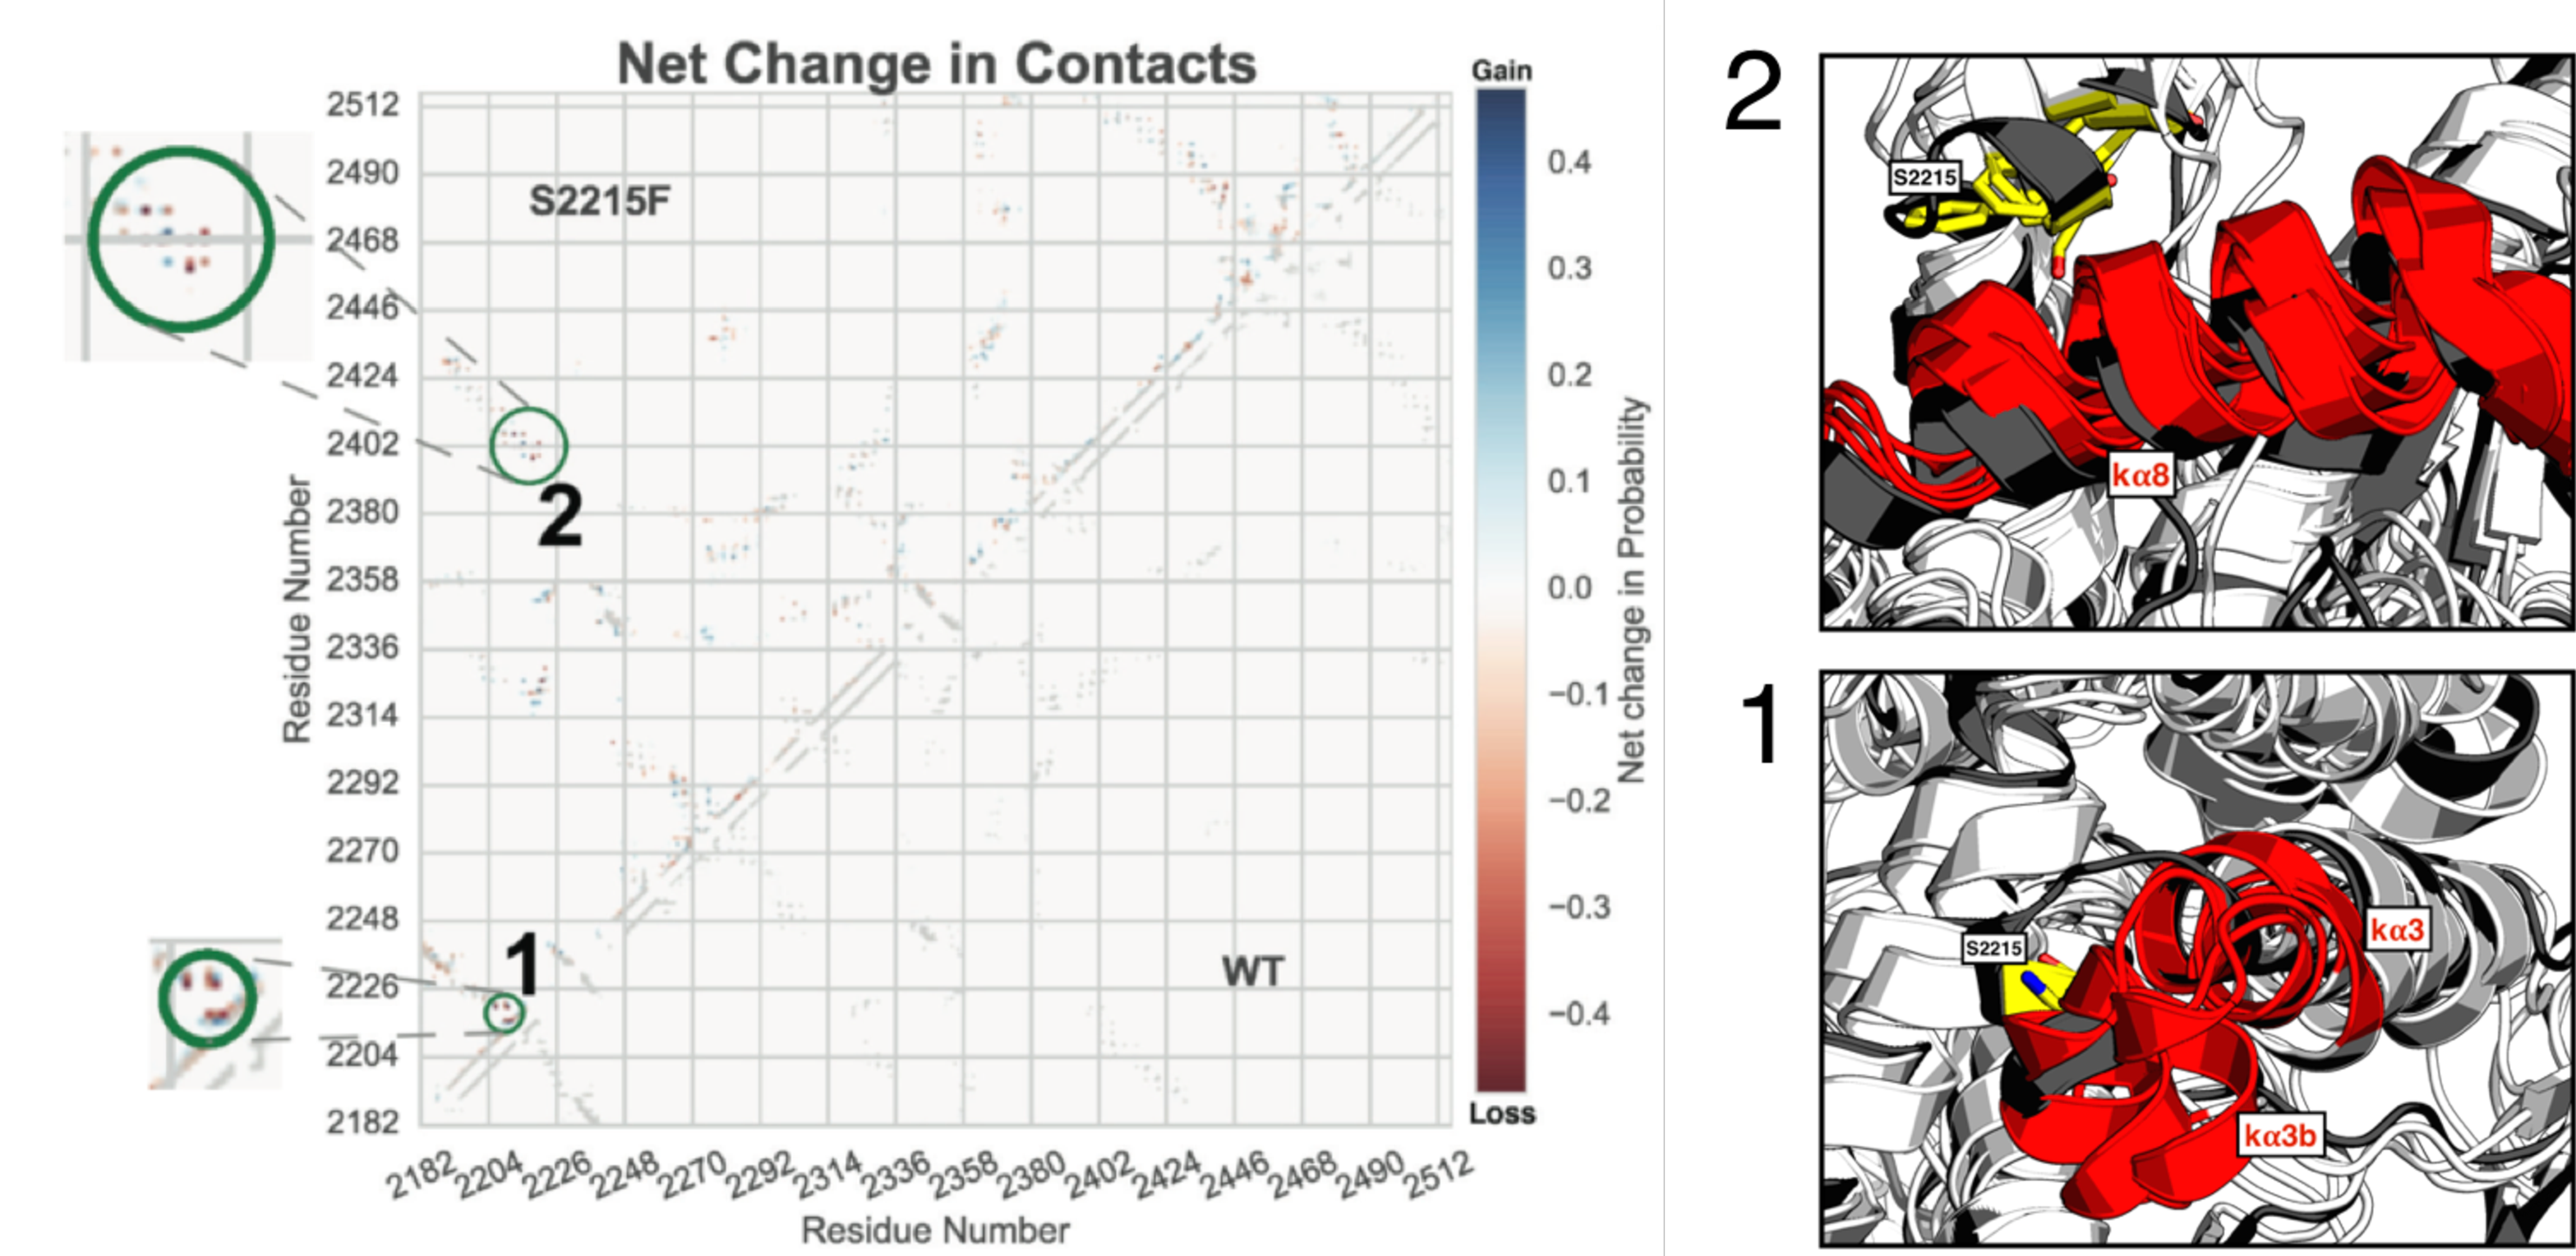
\includegraphics[width=1.0\linewidth]{figures/mtor-fig4.pdf}
		\caption[Missense mutations can perturb local structure]{
		{\bf Missense mutations can perturb local structure}
		 {\bf Left} Contact map showing the difference in probability of forming a contact between WT and mutant S2215F for Kinase Domain residues. {\bf Right} Regions one and two highlighted in contact map, showing a structural perturbation in indicated helices. Starting structure is shown in gray, the residues indicated in the contact map are shown in red and residue 2215 is shown in yellow. All trajectories started from PDB: 4JSV. \bf{This left panel of this figure is a modified version of a figure that appears in~\citep{Xu:2016fw}. Reprinted with permission of James Hsieh and the Journal of Clinical investigation}
	}
	\label{fig:mtor-figure4}
\end{figure}
\end{landscape}

\begin{landscape}
	\begin{figure}[p]
		\centering
		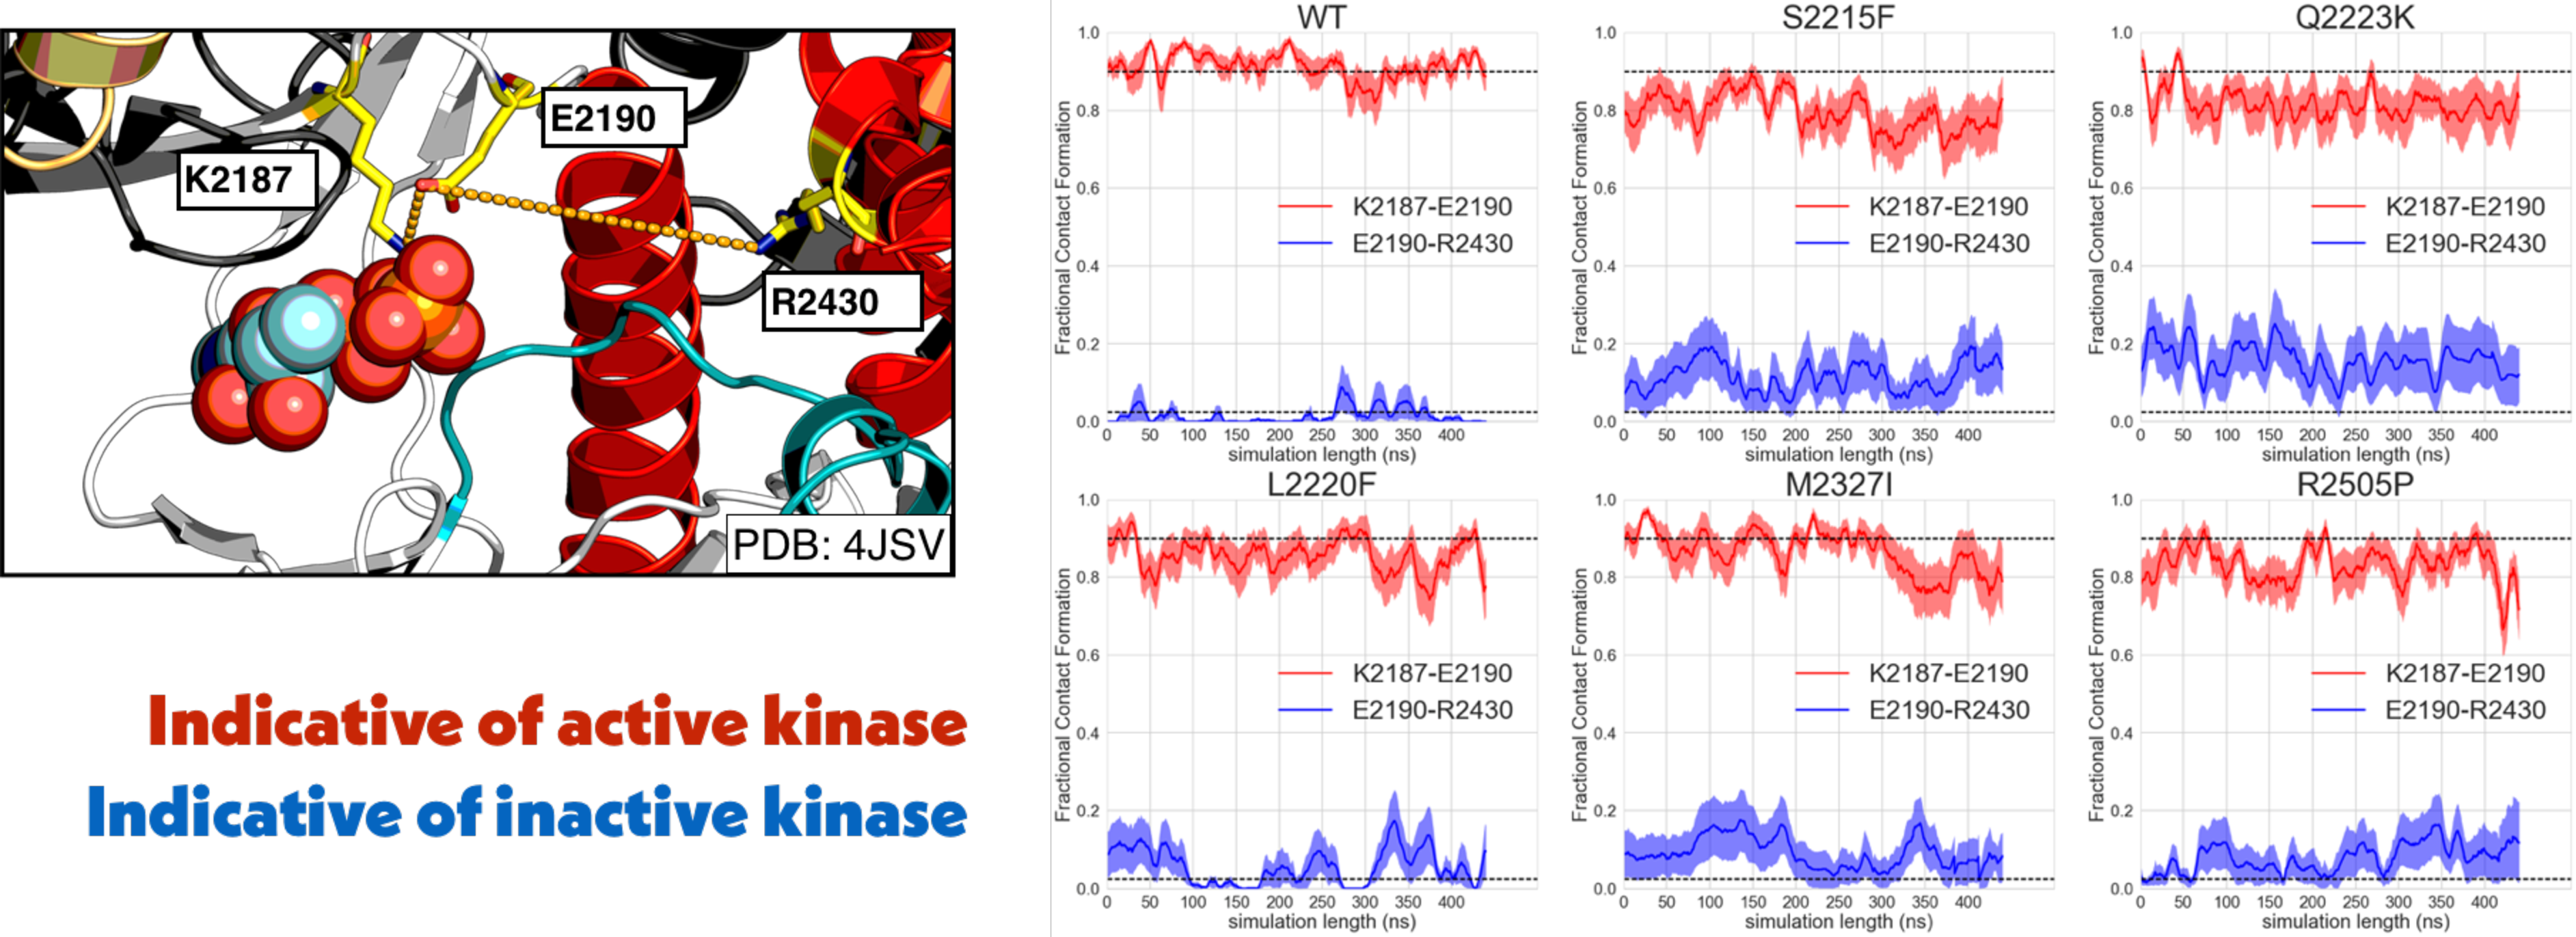
\includegraphics[width=1.0\linewidth]{figures/mtor-fig5.pdf}
		\caption[Missense mutations do not shift the population of the active conformation]{
			{\bf Missense mutations do not shift the population of the active conformation}
			{\bf Right} Fractional contact formation analysis for 20 500ns trajectories, analyzed in 20ns sliding window chunks. Contacts cutoff at 4Å for closest heavy atom.  Plotted is the mean $\pm$ SEM. The dashed lines represent the proportion roughly populated in the WT simulations. {\bf Left} Illustration of the bond formed between K2187 and E2190 (red) or E2190 and R2430 (blue). ATP is shown in spheres. The kinase domain (white) is shown with the activation loop (teal) and the $\alpha$ helices (red). The FRB domain is shown in gold. 
			}
		\label{fig:mtor-figure5}
	\end{figure}
\end{landscape}

\begin{landscape}
	\begin{figure}[p]
		\centering
		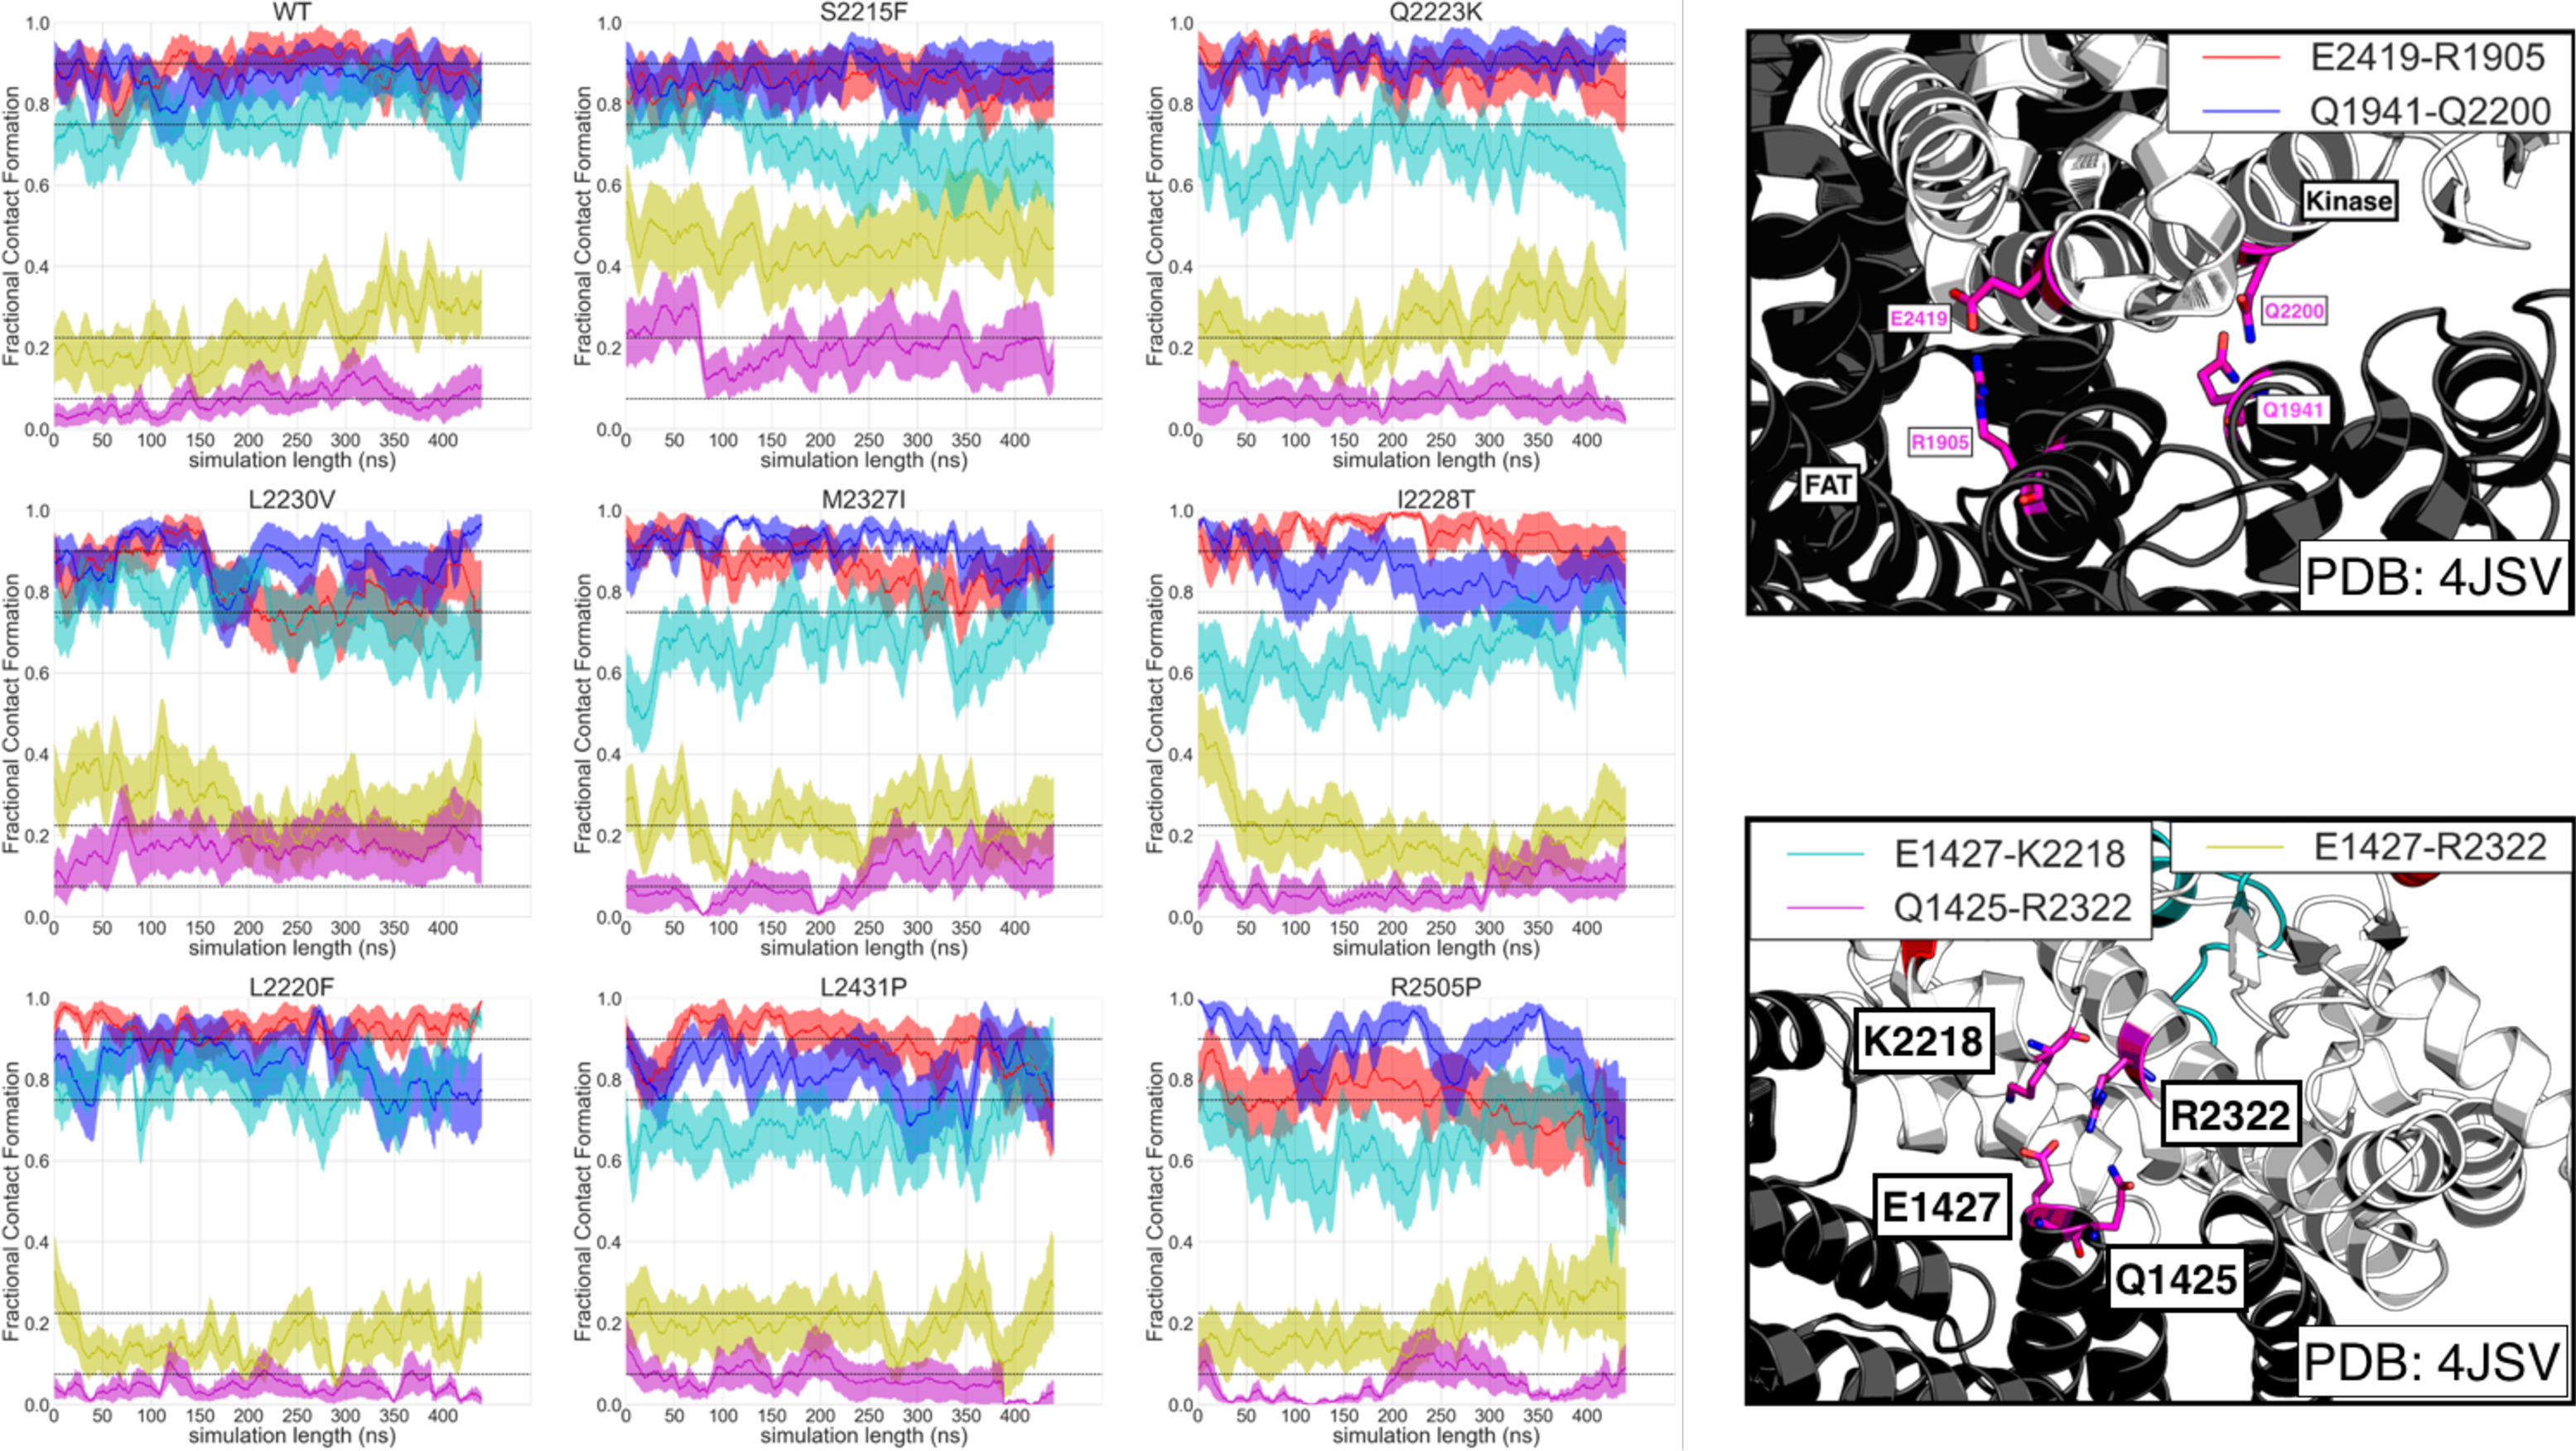
\includegraphics[width=1.0\linewidth]{figures/mtor-fig6.pdf}
		\caption[Missense mutations do not disrupt interactions between the kinase and FAT domains]{
			{\bf Missense mutations do not disrupt interactions between the kinase and FAT domains}
			{\bf Left} Fractional contact formation analysis for 20 500ns trajectories, analyzed in 20ns sliding window chunks. Contacts cutoff at 4Å for closest heavy atom.  Plotted is the mean $\pm$ SEM. The dashed lines represent the proportion roughly populated in the WT simulations. {\bf Right} Illustration of the distances being plotted between E2419 and R1905 (red), Q1941 and 2200 (blue), E1147 and K2218 (cyan), Q1425 and R2322 (magenta), or E1427 and R2322 (yellow) . ATP is shown in spheres. The kinase domain (white) interacts with the FAT domain (black) through salt bridges and hydrogen bonds formed by the highlighted residues (magenta) 
		}
		\label{fig:mtor-figure6}
	\end{figure}
\end{landscape}

\begin{landscape}
	\begin{figure}[p]
		\centering
		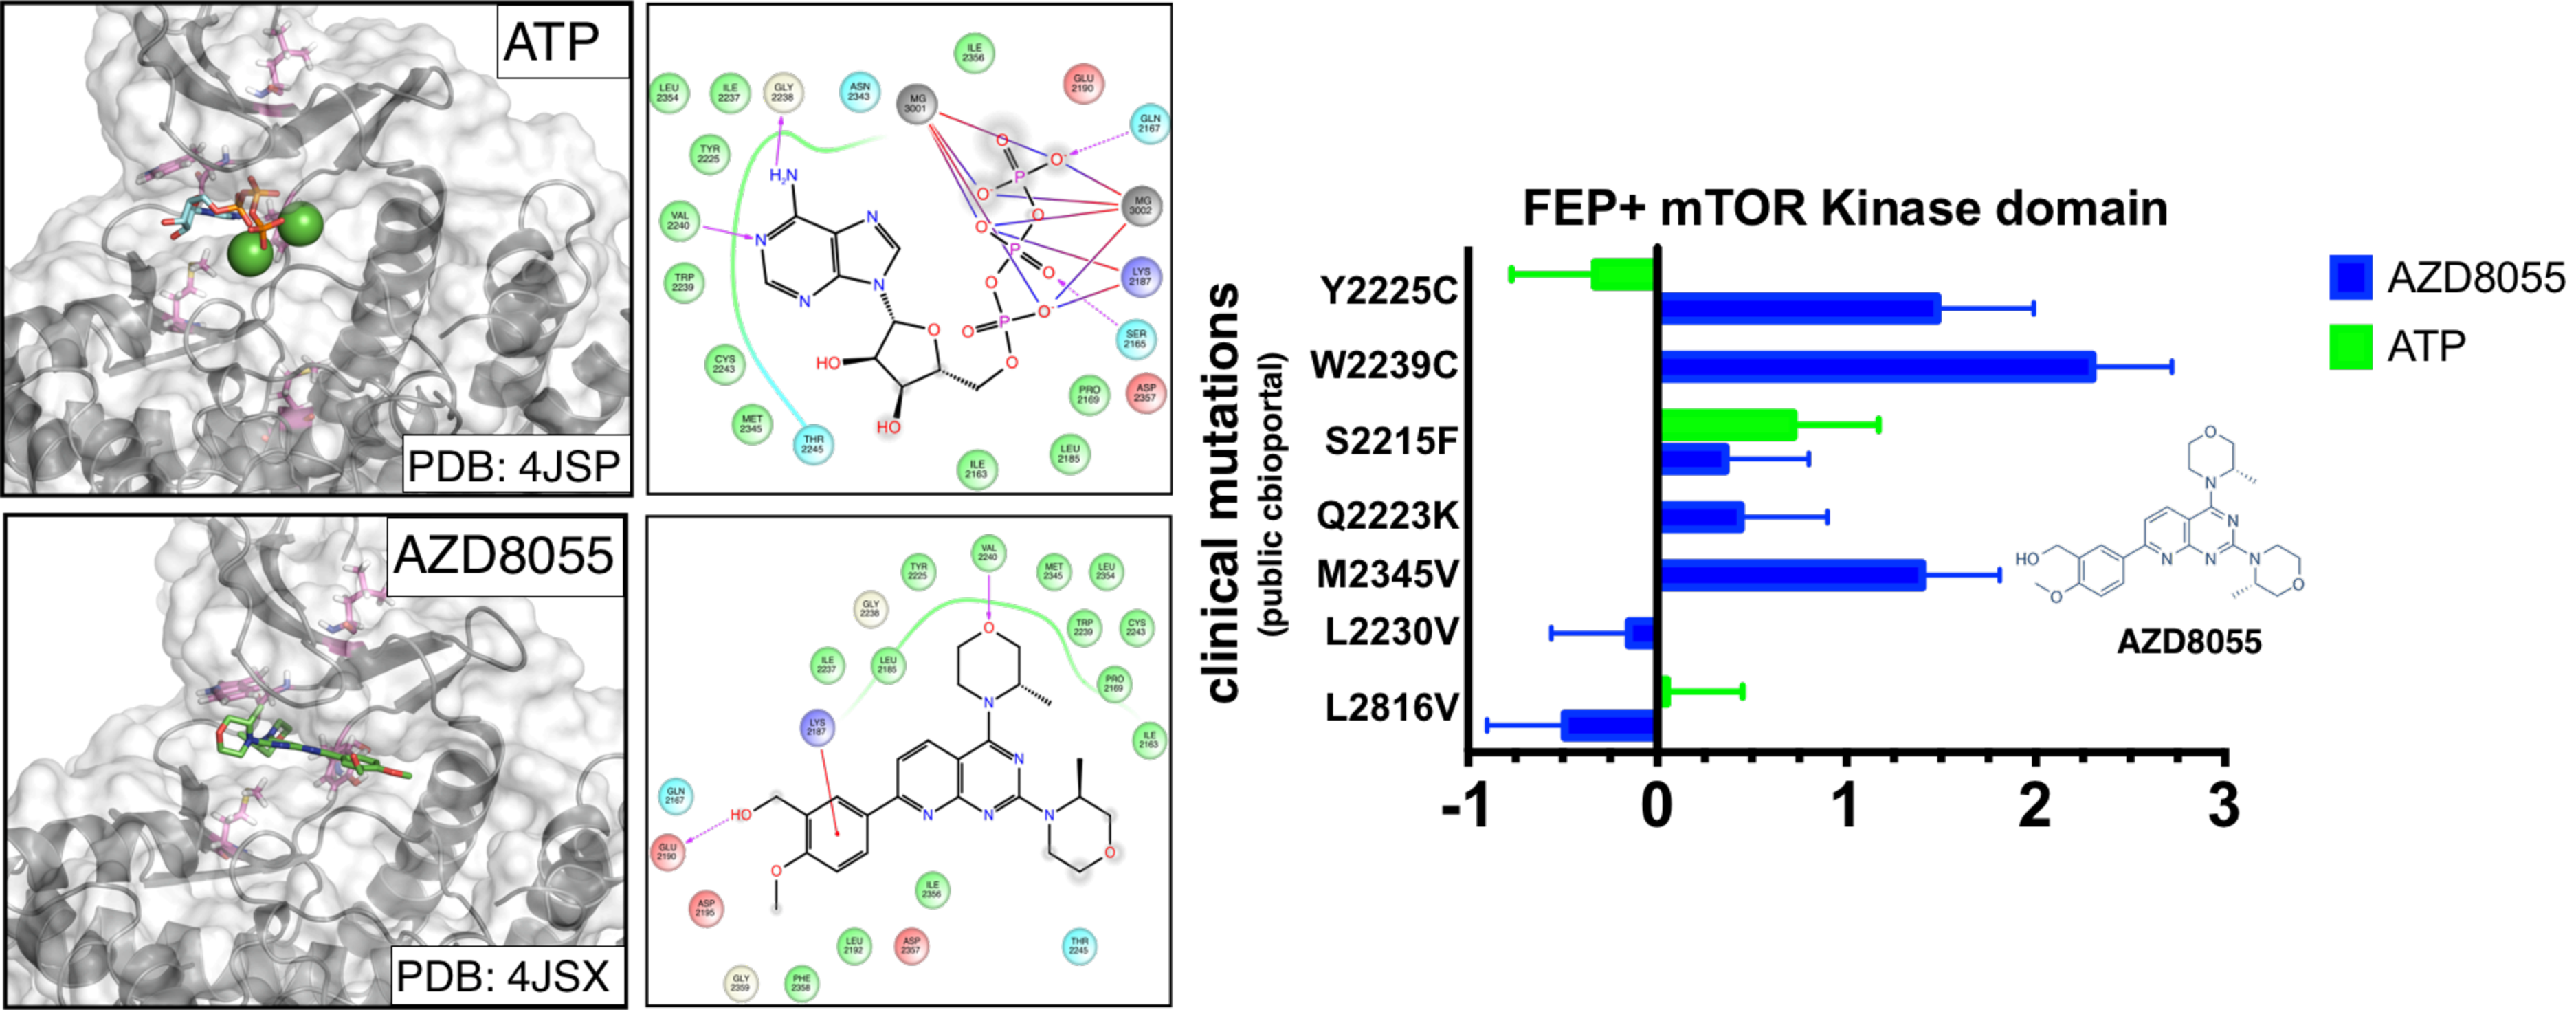
\includegraphics[width=1.0\linewidth]{figures/mtor-fig7.pdf}
		\caption[Free energy calculations identify potential resistance mutations]{
			{\bf Free energy calculations identify potential resistance mutations}
			{\bf Left} Structures and 2D interactions maps of ATP (top, PDBID: 4JSP) and AZD8055 (bottom, PDBID: 4JSX) docked to the kinase domain of mTOR. Magnesium ions are shown as green spheres.  {\bf Right} $\Delta \Delta G_{mutation}$ (x-axis) calculated for a number of clinically observed mTOR mutations(y-axis)~\citep{Zehir:Nat.Med.:2017} for ATP (green) and AZD8055 (blue). Error bars correspond to the BAR uncertainty estimate. 
		}
		\label{fig:mtor-figure7}
	\end{figure}
\end{landscape}

\section{Methods}
\subsection{Molecular dynamics simulations}
This work was performed and previously described in reference~\cite{Xu:2016fw}. The canonical wild-type mTOR sequence for the UniProt-annotated PI3K/PI4K domain span (residues 2182-2516) was modeled onto the X-ray structure of mTOR from chain A of
RCSB entry 4JSN using the Ensembler automated simulation setup tool~\citep{Parton:2016cc} with default parameters. All residues were assigned default protonation states typical of pH 7.4. The AMBER 99SB-ILDN~\citep{LindorffLarsen:2010ei} forcefield was used for the protein along with the TIP3P solvent model~\citep{Jorgensen:1998fl} with neutralizing monovalent Na+ or Cl- counterions. The resulting simulation box had 80,983 atoms. The OpenMM 6.2 simulation package~\citep{Eastman:2017kn} was used for all minimization, equilibration, and production simulations. Equilibration simulations utilized Langevin dynamics with a timestep of 2 fs and collision rate of 20/ps, along with a Monte Carlo barostat with molecular scaling and update interval of 50 steps, with temperature and pressure control set to 300 K and 1 atm. Particle-mesh Ewald (PME) with default parameters was used for long-range electrostatic treatment, direct-space and Lennard-Jones interactions were truncated at 9 A, and a long-range dispersion correction was employed. Bonds to hydrogen were constrained using CCMA~\citep{Eastman:2010hq} using the default tolerance of 1e-5, and waters were rigidly constrained using SETTLE~\citep{Miyamoto:1992fx}. The Ensembler package~\citep{Parton:2016cc} handles energy minimization and refinement in implicit solvent followed by a short minimization and equilibration step in explicit solvent prior to production simulations.
Production simulations of the wild-type kinase domain were run on Folding@home~\citep{Shirts:2000du} using a simulation core based on OpenMM 6.2 and the same simulation parameters, with the exception of a reduced collision rate of 1/ps. The structure obtained after 589.5 ns---which had relaxed much of the initial loop-modeling-induced structural artifacts---was used as a starting model for further modeling of mutations and subsequent production simulations.
To model mTOR mutants and wild-type kinase domain behavior, PDBFixer v1.2~\citep{Eastman:2013bo}, part of the Omnia molecular simulation suite, was used to generate mutant versions of the mTOR kinase domain using the relaxed wild-type structure. Subsequent simulation steps utilized reaction-field electrostatics with a cutoff of 10A in place of PME to allow longer trajectories to be generated. Proteins were resolved in TIP3P water with NaCl counterions to neutralize the system and produce an environment of approximately 150 mM NaCl to using a padding of 11A around the kinase, resulting in systems of approximately 81K atoms. Langevin dynamics with a collision rate of 5/ps was used for subsequent production simulations of mutant and wild-type kinase domains, which also employed a simulation core based on OpenMM 6.2 on Folding@home. Simulation boxes were energy minimized with the OpenMM LocalEnergyMinimizer facility before subjecting them to subsequent dynamics.
Ten replicate simulations of each mutant simulation box were run on Folding@home, with each replicate receiving a unique random number seed ensuring rapid decorrelation of trajectories. Nine out of ten trajectories were 501 nanoseconds of simulation, and one trajectory was 471 nanoseconds long. The initial 100 ns of each simulation were discarded and subsequent simulation data was analyzed for structural alternations indicative of rapid mutation- induced conformational changes.
Conformational changes were detected by generating a contact map, which shows the net change in the probability of forming a contact between a pair of residues from wild-type to mutant. To calculate these probabilities, mdtraj~\citep{McGibbon:2015fv} was first used to calculate the distance between every residue pair based on the closest heavy atoms in each frame of the simulations after 100 ns. Using 5 angstroms as the threshold at which a contact was formed, the number of frames in which a contact was formed was divided by the total number of frames for each simulation, giving a probability for each residue pair in that simulation which could be averaged over the number of replicates per mutant. The wild-type probability was subtracted from the mutant, giving a net change in probability to form a contact for each residue pair in the protein. The structural images were generated using PyMOL to visually inspect areas of interest identified by the contact map over the course of each simulation.

\subsection{Contact Map Analysis}
This work was performed and previously described in reference~\cite{Xu:2016fw}. The individual net changes in average contact probabilities following 100 ns of relaxation were computed as the difference in average contact probabilities between mutant and wild-type simulations. For each kinase, the average contact probability was computed as the fraction of snapshots in which the contact was made, where all frames (after discarding the initial 100 ns/trajectory) were averaged over the ten replicate trajectories initiated from each kinase mutant or wild-type simulation box using different initial velocities and random number seeds. The net change in probabilities are reported plus or minus a standard error, which is calculated as stddev/sqrt(N), where N=10 is the number of replicate trajectories.

\subsection{Mean Contact formation over time}
The fractional contact formation was calculated for 20 replicate 500ns trajectories. Analysis was carried out using 20ns sliding window chunks, with a single frame step (2fs) between each window.  Contact cutoff at 4$\AA$ for closest heavy atom.  Plotted is the mean $\pm$ SEM, calculated as in Equation~\ref{eq15}

\begin{equation}\label{eq14}
\sigma = \sqrt{\frac{ \sum^n (X_i - \mu_x)^2}{n-1}}
\end{equation}

\begin{equation}\label{eq15}
\text{SEM} = \frac{\sigma}{\sqrt{n}}
\end{equation}

Where $\sigma$ in Equation~\ref{eq14} is the standard deviation, $X_i$ fractional contact for a frame $i$, $\mu$ is the mean fractional contact for a 20ns window, and n is the total number of frames in that sliding window. 

\subsection{Alchemical free energy calculations}
\subsubsection{Structure and Ligand Preparation}
Structures for mTOR (4JSP~\citep{Yang:2013gaa} (ATP) and 4JSX~\citep{Yang:2013gaa} (AZD8055)) were downloaded from the PDB~\citep{Berman2002-hg}.
Models were prepared from chain A of  each structure using Schr{\"o}dinger's PrepWizard (2016-1)~\citep{Sastry2013-ax}. All other chains were deleted. PrepWizard was used to add in hydrogens at pH 7.4 for both protein residues and the cocrystallized ligand. The protonation state of the cocrystallized ligand was assigned the lowest energy state using Epik at pH $7.4\pm2$. Hydrogen bonding was optimized using PROPKA at pH $7.4\pm2$. Each of the structures was minimized using OPLS3~\citep{Harder:J.Chem.TheoryComput.:2016} and an RMSD convergence cutoff of 0.3$\AA$. The missing loops, due to their large size, were not modeled in, and were capped by PrepWizard. 

ATP and AZD8055 were prepared for docking using Schr{\"o}dinger's LigPrep (2016-1). 3D structures were generated using OPL3, and ionization state determined by Epik at pH $7.4\pm2$. All other settings were left on default. The lowest Epik state penalty state was selected for each ligand. 

\subsubsection{Docking}
ATP and AZD8055 were docked into 4JSP and 4JSX, respectively, using Schr{\"o}dinger's GLIDE (2016-1)~\citep{Friesner:2004hm,Halgren:2004dr,Friesner:2006cp}. The receptor grid was generated centered on the cocrystallized ligand using the default settings of the Receptor Grid Generation panel. None of the rotatable groups were allowed to rotate to improve computational efficiency. The ligands were docked into these receptor grids using the extra precision (XP) protocol. Ligand sampling was set to flexible, allowing for nitrogen inversions and sampling of different ring conformations. Epik state penalties were added to the docking score, although only one input for each ligand was used. A post docking minimization was performed on the top 5 poses for each ligand. The docking protocol was set to write out only the best pose for each ligand, on the basis of the docking score after minimization. 

\subsubsection{Protein mutation FEP+}
Protein mutation FEP+~\citep{Wang2015-cn,Hauser:2018vz,Abel:2017jt} was used to calculate $\Delta \Delta G_{mutation}$ for both ATP and AZD8055 structures for each mutation. The models generated above were parameterized using the default OPLS3 forcefield~\citep{Harder2016-zn} that shipped with Maestro 2016-1. SPC parameters were used for water. The FEP+ panel offers an automated workflow with only requires an input structure and specified mutations. The protocol carried out as described in reference~\cite{Hauser:2018vz}, with only single replicates performed. The reported uncertainties in each $\Delta \Delta G_{mutation}$ are the BAR uncertainty estimates. 


\section{Results}




\section{Conclusions}

\chapter{Predicting the impact of clinically-observed Abl inhibitors using physical modeling and biophysical experiments}
\section{Introduction}
Targeted kinase inhibitors are a major therapeutic class in the treatment of cancer.
A total of 43 selective small molecule kinase inhibitors have now been approved by the FDA~\citep{fda-approved-kinase-inhibitors}, including 34 approved to treat cancer, and perhaps 50\% of all current drugs in development target kinases~\citep{Santos:Nat.Rev.DrugDiscov.:2016}.
  Despite the success of selective inhibitors, the emergence of drug resistance remains a challenge in the treatment of cancer~\citep{Shah:CancerCell:2002,BUCZEK201431,huang2015mechanisms,Meyer2051,Davare29092015,VanAllen94,Rani3821,Holohan:Nat.Rev.Cancer:2013} and has motivated the development of second- and then third-generation inhibitors aimed at overcoming recurrent resistance mutations~\citep{Weisberg:Nat.Rev.Cancer:2007,Y.Lu:Curr.Med.Chem.:2011,Juchum:DrugResist.Updat.:2015,Song:ActaPharm.Sin.B:2015,Neel:NpjPrecis.Oncol.:2017}.   

  While a number of drug resistance mechanisms have been identified in cancer (e.g., induction of splice variants~\citep{Gruber2006}, or alleviation of feedback~\citep{Chandarlapaty:CancerCell:2011}), inherent or acquired missense mutations in the kinase domain of the target of therapy are a major form of resistance to tyrosine kinase inhibitors (TKI)~\citep{Knight:Nat.Rev.Cancer:2010,Holohan:Nat.Rev.Cancer:2013,Housman:Cancers:2014}.
  Oncology is entering a new era with major cancer centers now deep sequencing tumors to reveal genetic alterations that may render subclonal populations susceptible or resistant to targeted inhibitors~\citep{Zehir:Nat.Med.:2017}, but the use of this information in precision medicine has lagged behind. 
  It would be of enormous value in clinical practice if an oncologist could reliably ascertain whether these mutations render the target of therapy resistant or susceptible to available inhibitors; such tools would facilitate the enrollment of patients in mechanism-based basket trials~\citep{Redig::2015,Hyman:Cell:2017}, help prioritize candidate compounds for clinical trials, and aid the development of next-generation inhibitors. 

\subsection{The long tail of rare kinase mutations frustrates prediction of drug resistance}
  While some cancer missense mutations are highly recurrent and have been characterized clinically or biochemically, a long tail of rare mutations collectively accounts for the majority of clinically observed missense mutations (Figure \ref{abl-figure-1}a), leaving clinicians and researchers without knowledge of whether these uncharacterized mutations might lead to resistance.
  While rules-based and machine learning schemes are still being assessed in oncology contexts, work in predicting drug response to microbial resistance has shown that rare mutations present a significant challenge to approaches that seek to predict resistance to therapy~\citep{Pesesky:Front.Microbiol.:2016}.
    Clinical cancer mutations may impact drug response through a variety of mechanisms by altering kinase activity, ATP affinity, substrate specificities, and the ability to participate in regulatory interactions, compounding the difficulties associated with limited datasets that machine learning approaches face.
  In parallel with computational approaches, high-throughput experimental techniques such as MITE-Seq~\citep{Melnikov:NucleicAcidsRes.:2014} have been developed to assess the impact of point mutations on drug response. 
  However, the complexity of defining selection schemes that reliably correlate with \emph{in vivo} drug effectiveness and long turn-around times might limit their ability to rapidly and reliably impact clinical decision-making.

\begin{landscape}
\begin{figure}[p]
\centering
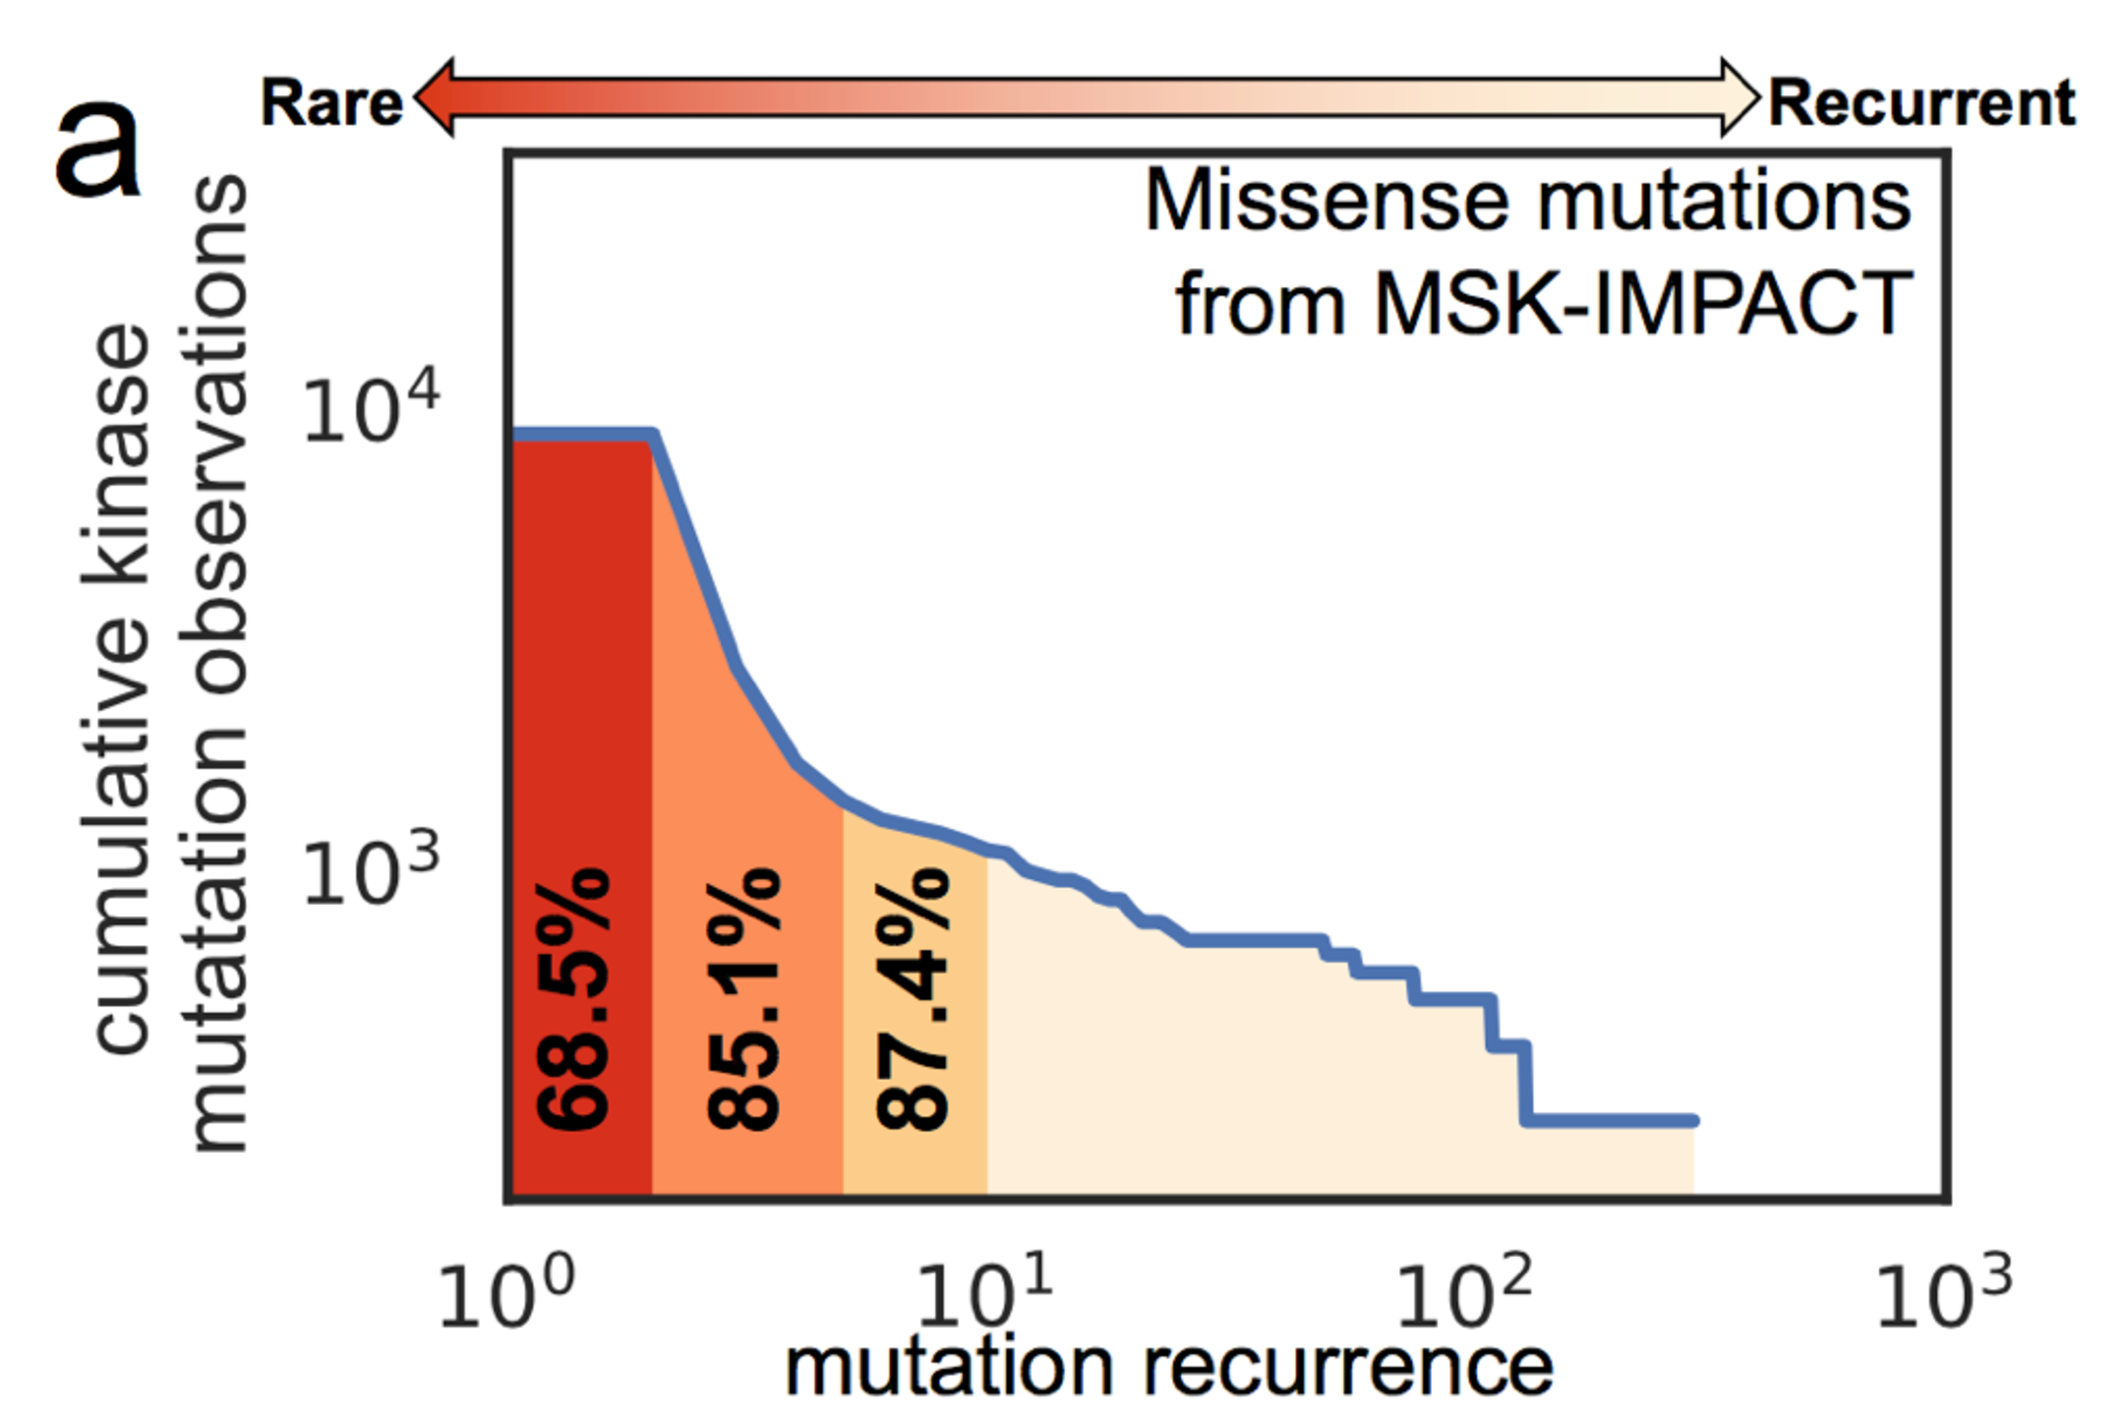
\includegraphics[width=0.90\linewidth]{figures/abl-figure-1.pdf}
\caption[Relative alchemical free-energy calculations can be used to predict affinity changes of FDA-approved selective kinase inhibitors arising from clinically-identified mutations in their targets of therapy.]{
{\bf Relative alchemical free-energy calculations can be used to predict affinity changes of FDA-approved selective kinase inhibitors arising from clinically-identified mutations in their targets of therapy.}
\emph{(a)}
Missense mutation statistics derived from 10,336 patient samples subjected to Memorial Sloan
Kettering-Integrated Mutation Profiling of Actionable Cancer Targets (MSK-IMPACT) deep sequencing panel~\citep{Zehir:Nat.Med.:2017} show that 68.5\% of missense kinase mutations in cancer patients have never been observed previously, while 87.4\% have been observed no more than ten times; the vast majority of clinically observed missense kinase mutations are unique to each patient.
\emph{(b)} To compute the impact of a clinical point mutation on inhibitor binding free energy, a thermodynamic cycle can be used to relate the free energy of the wild-type and mutant kinase in the absence (top) and presence (bottom) of the inhibitor.
\emph{(c)} Summary of mutations studied in this work. 
Frequency of the wild-type (dark green) and mutant (green) residues for the 144 clinically-identified Abl mutations used in this study (see \TABLE{table-1} for data sources). 
Also shown is the frequency of residues within 5 {\AA} (light blue) and 8 {\AA} (blue) of the binding pocket. 
The ordering of residues along the x-axis corresponds to the increasing occurrence of residues within 5 {\AA} of the binding pocket.
The number of wild-type Phe residues (n=45) and mutant Val residues (n=31) exceeded the limits of the y-axis.
}
\label{fig:abl-figure-1}
\end{figure}
\end{landscape}


\subsection{Alchemical free-energy methods can predict inhibitor binding affinities}
    Physics-based approaches could be complementary to machine-learning and experimental techniques in predicting changes in TKI affinity due to mutations with few or no prior clinical observations.
    Modern atomistic molecular mechanics forcefields such as OPLS3~\citep{Harder:J.Chem.TheoryComput.:2016}, CHARMM~\citep{Huang:J.Comput.Chem.:2013}, and AMBER FF14SB~\citep{Maier:J.Chem.TheoryComput.:2015} have reached a sufficient level of maturity to enable the accurate and reliable prediction of receptor-ligand binding free energy.
    Alchemical free-energy methods permit receptor-ligand binding energies to be computed rigorously, including all relevant entropic and enthalpic contributions~\citep{Chodera:Curr.Opin.Struct.Biol.:2011}.
    Encouragingly, kinase:inhibitor binding affinities have been predicted using alchemical free-energy methods with mean unsigned errors of 1.0 kcal mol$^{-1}$ for CDK2, JNK1, p38, and Tyk2~\citep{Wang:J.Am.Chem.Soc.:2015,abel2017accelerating}.
    Beyond kinases, alchemical approaches have predicted the binding affinity of BRD4 inhibitors with mean absolute errors of 0.6 kcal mol$^{-1}$~\citep{Aldeghi:ChemSci:2016}.
	Alchemical methods have also been observed to have good accuracy (0.6 kcal mol$^{-1}$ mean unsigned error for Tyk2 tyrosine kinase) in the prediction of relative free energies for ligand transformations within a complex whose receptor geometry was generated using a homology model~\citep{cappel2016}.


\subsection{Alchemical approaches can predict the impact of protein mutations on free energy}
	Alchemical free-energy calculations have also been used to predict the impact of mutations on protein-protein binding~\citep{clark2017free} and protein thermostabilities~\citep{steinbrecher2017predicting}.
	Recent work has found that protein mutations can be predicted to be stabilizing or destabilizing with a classification accuracy of 71\% across ten proteins and 62 mutations ~\citep{Ford:J.Chem.Inf.Model.:2017}.  
    The impact of Gly to D-Ala mutations on protein stability was predicted using an alchemical approach with a similar level of accuracy~\citep{Zou:J.Am.Chem.Soc.:2016}.
	Recently, one study has hinted at the potential utility of alchemical free-energy calculations in oncology by predicting the impact of a single clinical mutation on the binding free energies of the TKIs dasatinib and RL45~\citep{mondal2016}.

  

\subsection{Assessing the potential for physical modeling to predict resistance to FDA-approved TKIs}
  Here, we ask whether physical modeling techniques may be useful in predicting whether clinically-identified kinase mutations lead to drug resistance or drug sensitivity.
   We perform state-of-the-art relative alchemical free-energy calculations using FEP+~\citep{Wang:J.Am.Chem.Soc.:2015}, recently demonstrated to achieve sufficiently good accuracy to drive the design of small-molecule inhibitors for a broad range of targets during lead optimization~\citep{Lovering:ChemMedChem:2016,Chodera:Curr.Opin.Struct.Biol.:2011,Wang:J.Am.Chem.Soc.:2015,abel2017accelerating}, to calculate the effect of point mutation on the binding free energy between the inhibitor and the kinase receptor (Figure ~\ref{fig:abl-figure-1}b).
   %\FIG{figure-1}b depicts the thermodynamic cycle that illustrates how we used relative free energy calculations to compute the change in ligand binding free energy in response to the introduction of a point mutation in the kinase (\FIG{figure-1}c).
  We compare this approach against a fast but approximate physical modeling method implemented in Prime~\citep{Rapp:J.Chem.Inf.Model.:2011} (an MM-GBSA approach) in which an implicit solvent model is used to assess the change in minimized interaction energy of the ligand with the mutant and wild-type kinase.
  We consider whether these methods can predict a ten-fold reduction in inhibitor affinity (corresponding to a binding free energy change of 1.36 kcal mol$^{-1}$) to assess baseline utility.
  As a benchmark, we compile a set of reliable inhibitor $\Delta$pIC$_{50}$ data for 144 clinically-identified mutants of the human kinase Abl, an important oncology target dysregulated in cancers like chronic myelogenous leukemia (CML), for which six~\citep{fda-approved-kinase-inhibitors} FDA-approved TKIs are available.
  While $\Delta$pIC$_{50}$ can approximate a dissociation constant $\Delta K_{D}$, other processes contributing to changes in cell viability might affect IC$_{50}$ in ways that are not accounted for by a traditional binding experiment, motivating a quantitative comparison between $\Delta$pIC$_{50}$ and $\Delta K_{D}$.
  The results of this benchmark demonstrate the potential for FEP+ to predict the impact that mutations in Abl kinase have on drug binding, and a classification accuracy of $88_{82}^{93}$\%  (for all statistical metrics reported in this paper, the 95\% confidence intervals (CI) is shown in the form of ($x^{upper}_{lower}$)), an RMSE of $1.07_{0.89}^{1.26}$ kcal mol$^{-1}$, and an MUE of $0.79_{0.67}^{0.92}$ kcal mol$^{-1}$ was achieved. 
  
\subsection{A benchmark of $\Delta$pIC$_{50}$s for predicting mutational resistance} 
  To construct a benchmark evaluation dataset, we compiled a total of 144  $\Delta$pIC$_{50}$ measurements of Abl:TKI affinities, summarized in Table \ref{tab:table-1}, taking care to ensure all measurements for an individual TKI were reported in the same study from experiments run under identical conditions.
  131 $\Delta$pIC$_{50}$ measurements were available across the six TKIs with available co-crystal structures with wild-type Abl---26 for axitinib and 21 for bosutinib, dasatinib, imatinib, nilotinib, and ponatinib.
  13 $\Delta$pIC$_{50}$ measurements were available for the two TKIs for which docking was necessary to generate Abl:TKI structures---7 for erlotinib and 6 for gefitinib. 
  For added diversity, this set includes TKIs for which Abl is not the primary target---axitinib, erlotinib, and gefitinib.
  All mutations in this benchmark dataset have been clinically-observed (Table \ref{tab:table-1}). Due to the change in bond topology required by mutations involving proline, which is not currently supported by the FEP+ technology for protein residue mutations, the three mutations H396P (axitinib, gefitinib, erlotinib) were excluded from our assessment. As single point mutations were highly represented in the Memorial Sloan
Kettering-Integrated Mutation Profiling of Actionable Cancer Targets (MSK-IMPACT) study analyzed in Figure~\ref{fig:abl-figure-1}a, we excluded double mutations from this work. However, the impact of mutations from multiple sites can potentially be modeled by sequentially mutating each site and this will be addressed in future work.

%
%
%

%
%  TABLE 1
\begin{landscape}
\begin{table}[p]
\centering
\caption[Public $\Delta$pIC$_{50}$ datasets for 144 Abl kinase mutations and eight tyrosine kinase inhibitors (TKIs) with corresponding wild-type co-crystal structures]{
\label{tab:table-1}
{\bf Public $\Delta$pIC$_{50}$ datasets for 144 Abl kinase mutations and eight tyrosine kinase inhibitors (TKIs) with corresponding wild-type co-crystal structures used in this study}
}
% Use "S" column identifier to align on decimal point 
\setlength{\tabcolsep}{4pt}
%\rowcolors{2}{gray!25}{white}
\begin{tabularx}{\textwidth}{X c c X X S S S}
\toprule
			&				 		&			& 			&				& {(kcal mol$^{-1}$)}  										&										& {(kcal mol$^{-1}$)}		\\
{\bf TKI}	& {\bf N}$_\mathrm{mut}$& {\bf R}	& {\bf S}	& {\bf PDB}		& {$|\Delta G_\mathrm{max} - \Delta G_\mathrm{min}|$}	& {\bf Source}							& {$\Delta G_\mathrm{WT}$} \\
\toprule
axitinib	& 26					& 0			& 26		& 4wa9          & 2.05    												& \cite{Pemovska:Nature:2015}			& -8.35		\\
bosutinib	& 21					& 4			& 17		& 3ue4         	& 2.79    												& \cite{Gozgit3992}						& -9.81		\\
dasatinib	& 21					& 5			& 16		& 4xey        	& 5.08    												& \cite{Gozgit3992}						& -11.94	\\
imatinib	& 21					& 5			& 16		& 1opj          & 2.16    												& \cite{Gozgit3992} 					& -9.19		\\
nilotinib	& 21					& 4			& 17		& 3cs9       	& 3.88    												& \cite{Gozgit3992} 					& -10.74	\\
ponatinib	& 21					& 0			& 21		& 3oxz        	& 1.00    												& \cite{Gozgit3992} 					& -11.70	\\
%
{\bf subtotal}& {\bf 131}			&{\bf 18}	&{\bf 113}	& 				& 	    												& 										&	\\
%
erlotinib	& 7 					& 1			& 6			& \it{Dock to 3ue4}	& 1.73    												& \cite{Davis:Nat.Biotechnol.:2011}		& -9.77		\\
gefitinib	& 6						& 0			& 6			& \it{Dock to 3ue4}	& 1.79    												& \cite{Davis:Nat.Biotechnol.:2011}		& -8.84		\\
%
{\bf total}	& {\bf 144}				&{\bf 19}	&{\bf 125}	& 				&														&										& 	\\
\bottomrule

\end{tabularx}
\small
\smallskip
\\
{\bf N}$_\mathrm{mut}$: Total number of mutants for which $\Delta$pIC$_{50}$ data was available.\\
Number of {\bf R}esistant, {\bf S}usceptical mutants using 10-fold affinity change threshold.\\
PDB: Source PDB ID, or \emph{Dock to 3ue4}, which used 3ue4 as the receptor for Glide-SP docking inhibitors without co-crystal structure.\\
$\Delta G_\mathrm{WT}$: Binding free energy of inhibitor to wild-type Abl, as estimated from IC$_{50}$ data.
\end{table}
\end{landscape}
%

Experimental $\Delta$pIC$_{50}$ measurements for wild-type and mutant Abl were converted to $\Delta\Delta$G in order to make direct comparisons between physics-based models and experiment.
  However, computation of experimental uncertainties were required to understand the degree to which differences between predictions and experimental data were significant.
  Since experimental error estimates for measured IC$_{50}$s were not available for the data in \TABLE{table-1}, we compared that data to other sources that have published IC$_{50}$s for the same mutations in the presence of the same TKIs (\FIG{figure-2}a,b,c).
  Cross-comparison of 97 experimentally measured $\Delta\Delta$Gs derived from cell viability assay IC$_{50}$ data led to an estimate of experimental variability of $0.32^{0.36}_{0.28}$ kcal mol$^{-1}$ root-mean square error (RMSE) that described the expected repeatability of the measurements.
  Because multiple factors influence the IC$_{50}$ aside from direct effects on the binding affinity---the focus of this study---we also compared $\Delta\Delta$Gs derived from $\Delta$pIC$_{50}$s with those derived from binding affinity measurements ($\Delta K_{d}$) for which data for a limited set of 27 mutations was available (Figure~\ref{abl-figure-2}d); the larger computed RMSE of $0.81^{1.04}_{0.59}$ kcal mol$^{-1}$ represents an estimate of the lower bound of the RMSE to the IC$_{50}$-derived $\Delta\Delta$Gs that we might hope to achieve with FEP+ or Prime, which were performed using non-phosphorylated models, when comparing sample statistics directly.
In comparing 31 mutations for which phosphorylated and non-phosphorylated $\Delta K_{d}$s were available, we found a strong correlation between the $\Delta\Delta$Gs derived from those data (r=0.94, Supplementary Figure \ref{fig:figure-si-1}); the statistics of that comparison are similar to those of the inter-lab variability comparison.



%
%  FIGURE 2
%
\begin{landscape}
\begin{figure}[p]
\centering
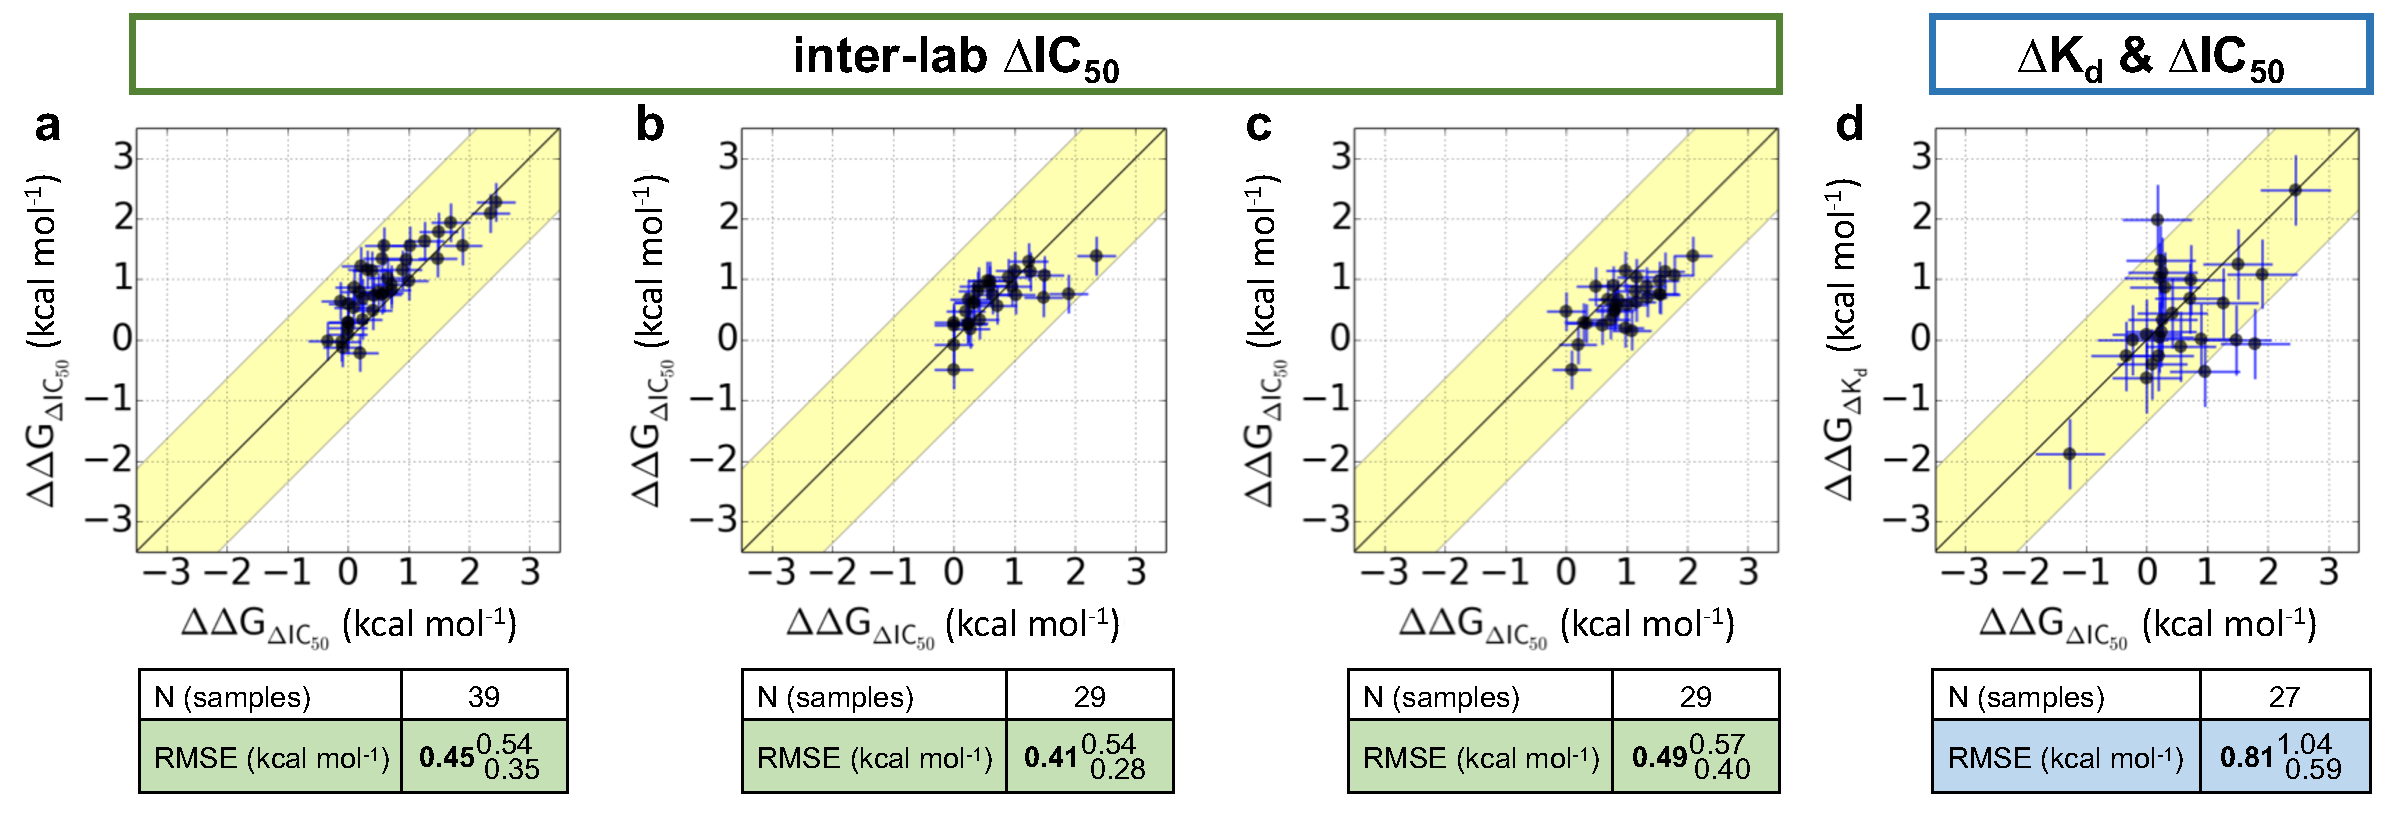
\includegraphics[width=0.95\linewidth]{figures/abl-figure-2.pdf}
\caption[Cross-comparison of the experimentally measured effects that mutations in Abl kinase have on ligand binding, performed by different labs.]{
{\bf Cross-comparison of the experimentally measured effects that mutations in Abl kinase have on ligand binding, performed by different labs.}
$\Delta\Delta$G was computed from publicly available $\Delta$pIC$_{50}$ or $\Delta$p$K_{d}$ measurements and these values of $\Delta\Delta$G were then plotted and the RMSE between them reported.
({\bf a}) $\Delta$pIC$_{50}$ measurements (X-axis) from \protect\cite{Gozgit3992} compared with $\Delta$pIC$_{50}$ measurements (Y-axis) from \protect\cite{Soverini7374}.
({\bf b}) $\Delta$pIC$_{50}$ measurements (X-axis) from \protect\cite{Gozgit3992} compared with $\Delta$pIC$_{50}$ measurements (Y-axis) from \protect\cite{o2007bcr}.
({\bf c}) $\Delta$pIC$_{50}$ measurements (X-axis) from \protect\cite{Soverini7374} compared with $\Delta$pIC$_{50}$ measurements (Y-axis) from \protect\cite{o2007bcr}.
({\bf d}) $\Delta$pIC$_{50}$ measurements (X-axis) from \protect\cite{Gozgit3992} compared with $\Delta$p$K_{d}$ measurements (Y-axis) from \protect\cite{Davis:Nat.Biotechnol.:2011} using non-phosphorylated Abl kinase.
Scatter plot error bars in a,b,and c are $\pm$standard error (SE) taken from the combined 97 inter-lab $\Delta\Delta$Gs derived from the $\Delta$pIC$_{50}$ measurements, which was 0.32$_{0.28}^{0.36}$;
the RMSE was 0.45$_{0.39}^{0.51}$ kcal mol$^{-1}$. Scatter plot error bars in d are the $\pm$standard error (SE) of $\Delta\Delta$Gs derived from $\Delta$pIC$_{50}$ and $\Delta$p$K_{d}$ from a set of 27 mutations, which is 0.58$_{0.42}^{0.74}$ kcal mol$^{-1}$;
the RMSE was 0.81$_{0.59}^{1.04}$ kcal mol$^{-1}$.
}
\label{fig:abl-figure-2}
\end{figure}
\end{landscape}




\subsection{Summary of experimental data that is available and what needs to be done to make better information available}
\subsection{Open-source YANK/Amber forcefield stuff}


\bibliographystyle{vancouver-elife.bst}
\bibliography{albanese}
\end{document}
